\chapter{Appendix}

This section includes the source-code for the DSP Data Persistence, as well as
the experiments artifacts used. Each section details one single main artifact
used on the development of the component. However, only the main ones will be
added into this document, while the remainder can be downloaded directly from
the Subversion repository.

\section{The Data Sensor Platform (DSP)}
\label{sec:dsp-details}

The Data Sensor Platform, in short DSP Platform, is based on a micro-kernel
architecture developed on top of the Java modular framework called OSGi
\cite{osgi}. The platform represents the foundation of the execution of
NetBEAMS, since it is executed from an embedded hardware called Gumstix
\cite{gumstix} using a Linux operating system and on top of the Java Virtual
Machine (JVM). In order to transport data from sensors hosts to the network
sink, the use of a cellular connection is used to transport the collected data
from the senso devices using the HTTP Protocol, as described by
\citet{netbeams2009}. Figure \ref{fig:sf-netbeams-node} shows the
architecture of the inhanced node designed by the NetBEAMS research group.

\begin{figure}[h]
  \centering
  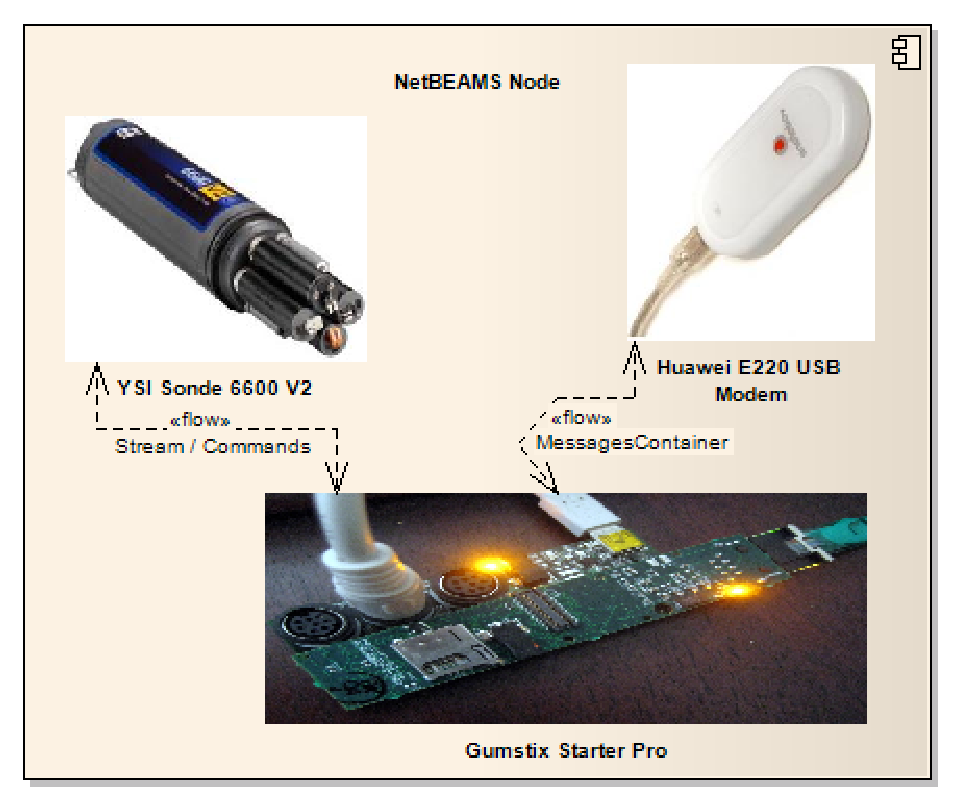
\includegraphics[scale=0.5]{../diagrams/DSP-Gateway-Node}
  \caption{The NetBEAMS Node enhancement with the Gumstix and the GSM Modem}
  \label{fig:sf-netbeams-node}
\end{figure}

The following list describes each of the devices in the NetBEAMS Node.

\begin{itemize}
  \item \textbf{YSI 6600EDS V2}: the YSI device is the regular sonde
  responsible for observing the environment. It is connected to the Gumstix
  embedded system, where the DSP is executed;
  \item \textbf{Gumstix console-vx}: it's a COTS ARM-based hardware that
  provides a computer-on-module environment for the development of small
  embedded systems. This is the main environment of data extraction and remote
  processing is accomplished. It runs a cross-compiled version of Linux Kernel
  2.6;
  \item \textbf{Huawei E220 USB Modem}: it is used to transfer the data from the
  Gumstix to the RTC Labs Data Center.
\end{itemize} 

The DSP runs inside of the embedded system Gumstix. The following sections
details its design and process for extracting data.

\subsection{The DSP System Design}

This section focus on the development of a Software Platform for the NetBEAMS
Gateway Embedded System, or on the system developed in the Gumstix device. As
shown in Figure \ref{fig:netbeams-software-stack}, the NetBEAMS Gateway Node is
an embedded system that contains a set of layer found in any computer.
However, each of the resources described from the system were customized for
the NetBEAMS system. The main components of such system can be summarized as
follows:

\begin{itemize}
  \item \textbf{Operating System}: it uses a cross-compiled Gentoo Linux, which
  supports a wide variety of development tools, including the Java Virtual Machine
  (JVM), the underlying platform system;
  \item \textbf{Java Virtual Machine}: it uses the JamVM, a ~200 KB version of
  the Sun Microsystems Java Virtual Machine, version 2.0;
  \item \textbf{OSGi Framework}: it uses the Knopflerfish implementation of the
  OSGi 4.1 specification. More details in the following sections.
  \item \textbf{DSP Platform and other Bundles}: The plug-and-play DSP
  Components are based on the OSGi bundles capabilities, which can reuse
  services registered in the OSGi framework.
\end{itemize}

\begin{figure}[h]
  \centering
  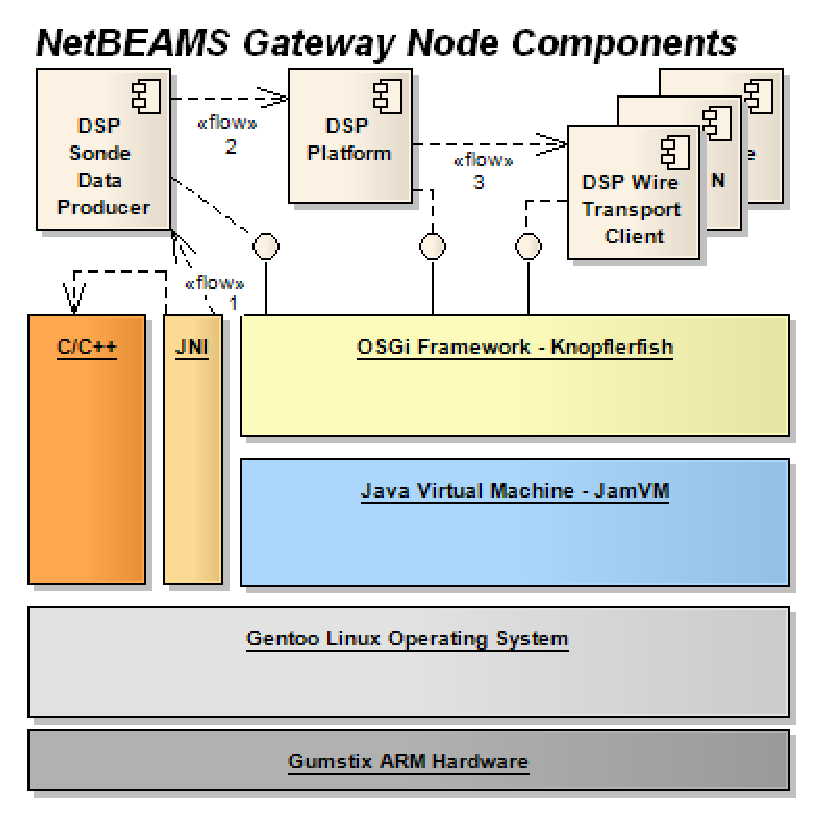
\includegraphics[scale=0.6]{../diagrams/NetBEAMS-Client-Node-Components}
  \caption{The NetBEAMS's Gumstix Software Stack}
  \label{fig:netbeams-software-stack}
\end{figure}

As depicted in Figure \ref{fig:netbeams-software-stack}, the DSP Sonde Data
Producer component opens a serial connection with the device through the Java
Native Interface (JNI) driver and produces the data flow 1. The data stream
format at this stage is as described on table \ref{tab:ysi-data-stream}.
Later, by parsing and transforming the data to DSP internal representation, it
sends the data to the DSP Platform as depicted on flow 2. Finally, the DSP
Platform decides to send the data to the DSP Wire Transport Client, as shown
on flow 3, by following rules defined by the system administrator. At this
point, the data is ready to be transmitted to the server, which is covered on
the following sections.

\subsection{The DSP Platform Architecture}
\label{sec:netbeams-architecture}

The architecture of the DSP, aligned with the OSGi capabilities, reuses the
Service-Oriented Architecture that can easily enable and disable plug-and-play
components. By following a publish-subscriber design-pattern \cite{gof}, the
service producer registers into the service broker while the consumer looks
for a given registered service in the Service Broker. For this reason, this
approach allows decoupled interoperability among modules as it is shown in
figure \ref{fig:publish-subscriber-pattern}.

\begin{figure}[h]
  \centering
  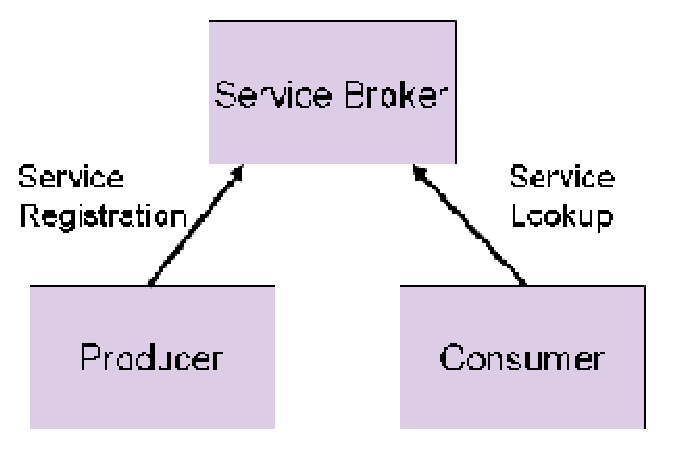
\includegraphics[scale=0.6]{../diagrams/publish-subscriber-pattern}
  \caption{The publish-subscriber design-pattern for services}
  \label{fig:publish-subscriber-pattern}
\end{figure}

The DSP infrastructure is based on a loosely-coupled architecture hosted in a
given host computer with an OSGi container, where the entire system is
composed by a set of plug-n-play OSGi modules. Each DSP component, as an
instance of an OSGi Module, can perform specialized tasks according to its
specification. In general, each DSP component can be categorized as follows:

\begin{itemize}
  \item \textbf{Data Producer (DP)}, whose main function is to produce data for
  the system;
  \item \textbf{Data Consumer (DC)}, whose main function is to consume the
  received data.
\end{itemize}

\begin{figure}[!b]
  \centering
  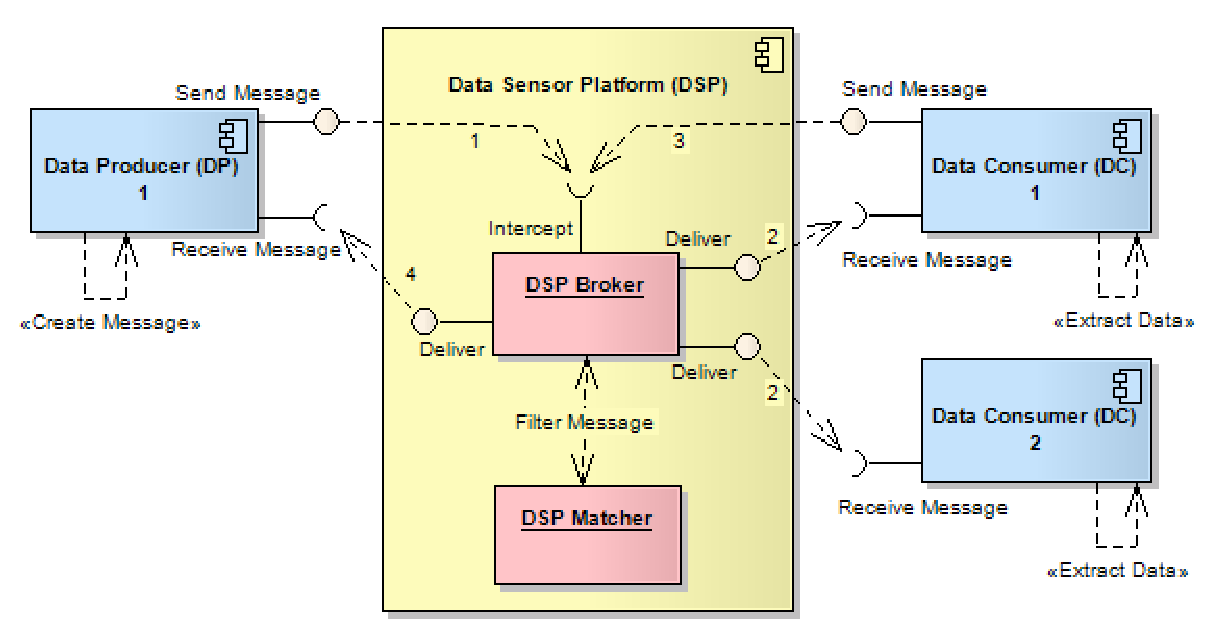
\includegraphics[scale=0.7]{../diagrams/DSP-Producers-Consumers-Components-Interactions}
  \caption{The basic architecture of a Data Sensor Platform (DSP)}
  \label{fig:DSP-Producers-Consumers-Components-Interactions}
\end{figure}

The Data Producers and Data Consumers exchange data through the DSP Message
Broker using a message unit called DSP Message. As it is depicted in figure
\ref{fig:DSP-Producers-Consumers-Components-Interactions}, a Data Producer
creates a set of one or more DSP Messages wrapped up in a DSP
MessagesContainer in order to be sent to the DSP Message Broker. When the
broker receives the set of DSP Messages, it requests a list of Data Consumers
to each of the DSP Messages based on rules managed by the DSP Matcher.
Whenever the broker acquires the list of Data Consumers, it delivers a copy of
the DSP Message to each of the Data Consumers in the receiving list. Upon the
DSP Message arrival, each Data Consumer can extract the actual data from the
DSPMessage. Finally, although the components can be distinguished between Data
Producers and Consumers, any of them are entitled to send and receive
administrative DSP Messages, which is covered in the following sections.

When the DSP Platform is installed into the OSGi framework, it follows the
OSGi specifications without any changes to remain it in the installed state.
In this way, it is important to note that the DSP Platform and its
plug-and-play components are directly mapped with the OSGi Framework as
follows:

\begin{itemize}
  \item \textbf{OSGi Bundle} = DSP Component Artifact in Jar format
  \begin{itemize}
    \item SondeDSPProducer.jar is the component developed for the YSI sonde
  \end{itemize}  
  \item \textbf{OSGi Activator} = DSP Component Activator
  \begin{itemize}
    \item Class specified in the MANIFEST.MF artifact (next sections)
  \end{itemize} 
  \item \textbf{OSGi Service Reference} = DSP Component Class
  \begin{itemize}
    \item  Class specified by the component author.
  \end{itemize}
\end{itemize}

The DSP Platform, along with the DSP Framework, are the only DSP Components
needed to be installed into the OSGi container. For this reason,the DSP
Platform is responsible to install and activate the additional DSP components
that makes part of the platform during the start up process, which leverages
its bootstrap process. Nevertheless, in order to automate the process of
automatic install and removal of the plug-and-play components, the DSP Platform
provides a deployment configuration file that describes which DSP components
must be installed with a given priority number. The name of this configuration
artifact is called config.xml (see listing \ref{file:dsp-config.xml}), and is
depicted by the XML Schema \cite{xml-schema} in figure
\ref{fig:dsp-config-schema}.

\begin{figure}[h]
  \centering
  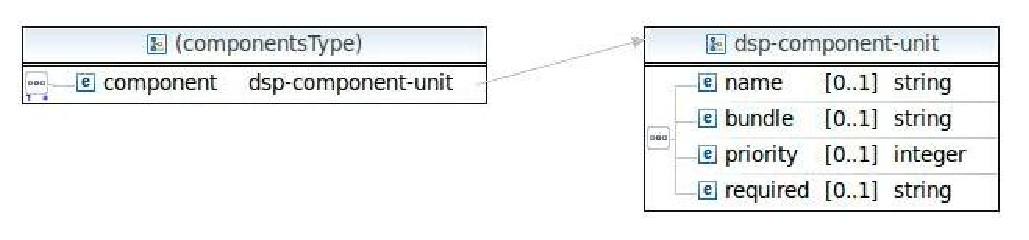
\includegraphics[scale=0.8]{../diagrams/config-schema}
  \caption{XML Schema for the main DSP deployment configuration artifact}
  \label{fig:dsp-config-schema}
\end{figure}

In order to show an example, consider the DSP Platform on the embedded system
Gumstix in Figure \ref{fig:sf-netbeams-node}. It is started by providing a
deployment configuration artifact config.xml included in the appendix. It lists
the components that the DSP Platform needs to install and load for its
operation. As it is shown, the DSPWireTransportClient and the DSPSondeProducer
are the identification of the components, followed by the name of the physical
file and an assigned loading priority. While the DSPWireTransportClient is
responsible for the serialization and deserialization of the DSP Messages
exchanged by the DSPSondeProducer and any remote DSP component. In this case,
the DSPSondeProducer is the DSP component responsible to collect measurement
data from the YSI Sonde and temporarily store them before being transmitted.

Therefore, in order to orchestrate the DSP Components together, the DSP
Platform component is responsible for installing and uninstalling during its
state "Starting" and "Stopping", respectively, as it is shown in figure
\ref{fig:DSPPlatform-Install-Usage-State-Diagram}. When the system
administrator starts the DSP Platform, it performs the regular OSGi procedures
to start the bundle. Up until that state, it will get the list of DSP
Components to be installed as described in the config.xml artifact, trying to
install each of them in an optimistic way. After that, it will continue on the
state "Active" until the system administrator decides to stop it.

\begin{figure}[!b]
  \centering
  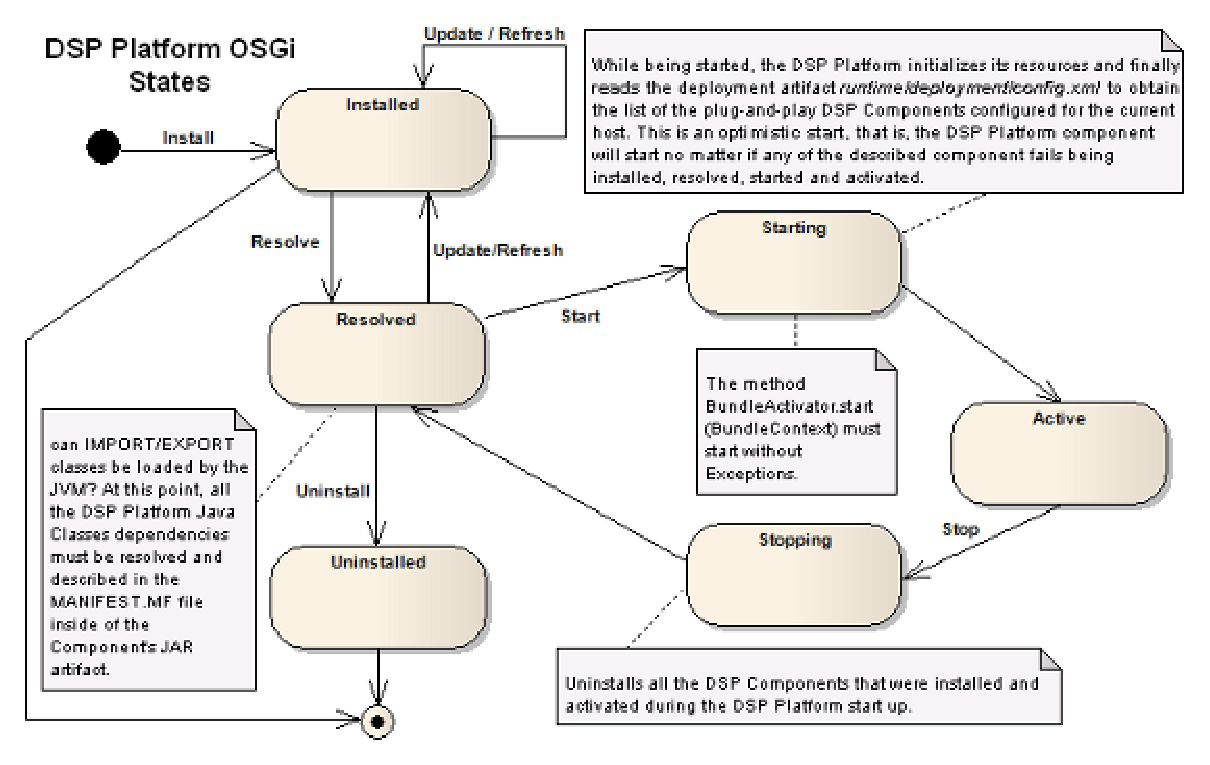
\includegraphics[scale=0.6]{../diagrams/DSPPlatform-Install-Usage-State-Diagram}
  \caption{The DSP Platform State Diagram}
  \label{fig:DSPPlatform-Install-Usage-State-Diagram}
\end{figure}

When the DSP Platform is on the Active state, it is ready to manage the DSP
Messages exchanges as described through figure
\ref{fig:DSP-Producers-Consumers-Components-Interactions}. The following
sections describe the participating classes in starting the DSP Platform and
its execution.

In a nutshell, the DSP Platform is an extension of the OSGi Platform, as it can
be seen in the UML Class Diagram \cite{uml} in figure
\ref{fig:DSP-Platform-Class-Diagram-Simple}. The class Activator contains a
unique instance of the Platform class, which contains instances of the classes
ComponentManager, Matcher, the MessageBroker and DSPContextImpl. The
DSPBundleController is the main instance that manages the plug-and-play DSP
components, and therefore, is tightly-coupled with the OSGi Framework classes.
Additionally, this class is part of the publish-subscriber design-pattern, as
it it implements the interfaces Bundle Listener and Service Listener, whose
responsibility is to track listens to the changes of the state of
ServicesReferences on the DSP Platform.

\begin{figure}[!t]
  \centering
  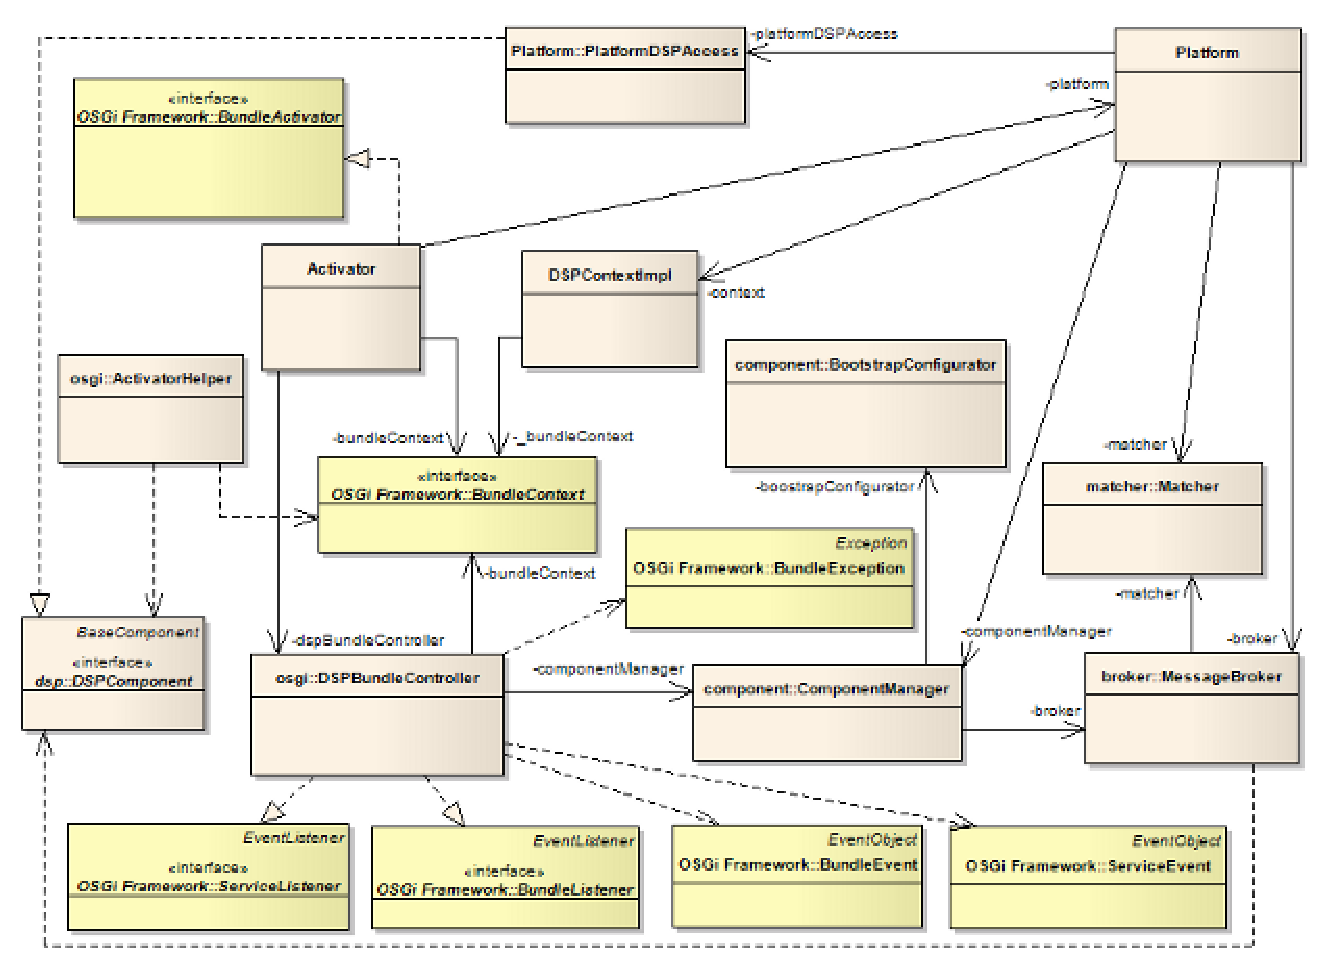
\includegraphics[scale=0.7]{../diagrams/DSP-Platform-Class-Diagram-Simple}
  \caption{The DSP Platform UML Class Diagram}
  \label{fig:DSP-Platform-Class-Diagram-Simple}
\end{figure}

\section{DSP Message and DSP Messages Container}
\label{sec:dsp-message}

As shown in the previous section, a DSP Message is the main unit of
communication among DSP Components. In a nutshell, a DSP Message can be seen
as an abstraction of an envelop containing the sections: a header and a body.
The former is used for identification and routing purposes, while the latter is
used to carry the payload of the message, that is, the collected data from
a sensor. Figure \ref{fig:DSP-Message-Representation} depicts the abstraction
of a DSP Message and its main components.

\begin{figure}[!b]
  \centering
  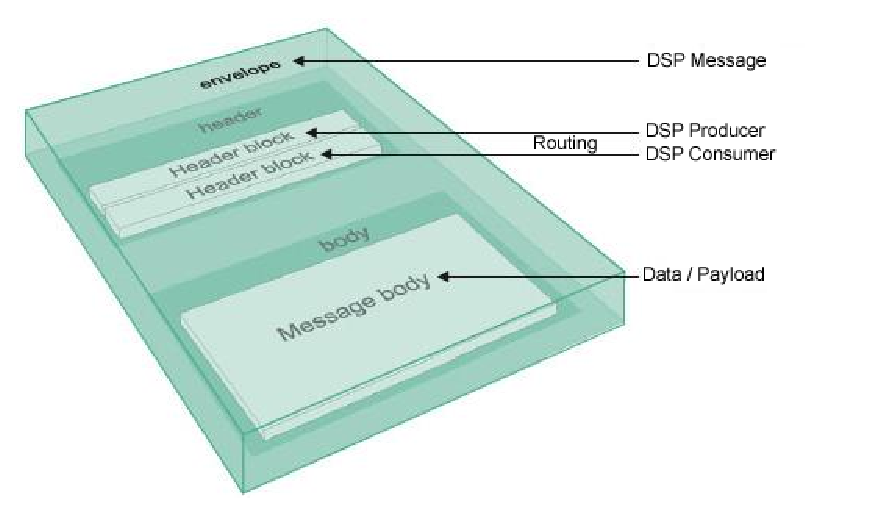
\includegraphics[scale=0.8]{../diagrams/DSP-Message-Representation}
  \caption{An Abstraction of a DSP Message and its components}
  \label{fig:DSP-Message-Representation}
\end{figure}

\begin{itemize}
  \item \textbf{Header} is composed by 2 blocks that identify the data
  producer and consumer of the message, as well as the time of creation, UUID,
  etc. It is an important piece of information for the data delivery and
  routing purposes.
  \item \textbf{Body} contains the payload of the message. This section carries
  the collected data from a sensor.
\end{itemize}

In general, the DSP Platform offers a veriety of types of DSP Messages for
different purposes. For example, any measurement data must be
wrapped up in a Measurement Message, while a Query Message is used to exchange
messages among the components for the purpose of management. In this way, the
main DSP Messages can be summarized as follows:

\begin{itemize}
  \item \textbf{Measurement Message} is used to transport any sensor collected
  data;
  \item \textbf{Query Message} is used to query a DSP component about its
  configuration properties;
  \item \textbf{Update Message} used to update a DSP component's configuration
  properties;
  \item \textbf{Acknowledgement Message} is used for the transport communication
  protocol, by acknowledging the reception of a DSP Message. More details in the
  Remote Data delivery section.
\end{itemize}

These DSP Classes and other can be seen in Figure the  UML Class
Diagram \cite{uml} of Figure \ref{fig:DSP-Messages-Classes}. Each DSP Message
contains an instance of a Header and Body. Whenever a DSP component is ready
to transmit messages, it wraps up the set of DSP Messages into the instance of
the Messages Container, which contains information about the collection of
messages being transmitted with its own identification. In this fashion, the
Messages Container is the main communication unit between 2 different DSP
Components.

\begin{figure}[!t]
  \centering
  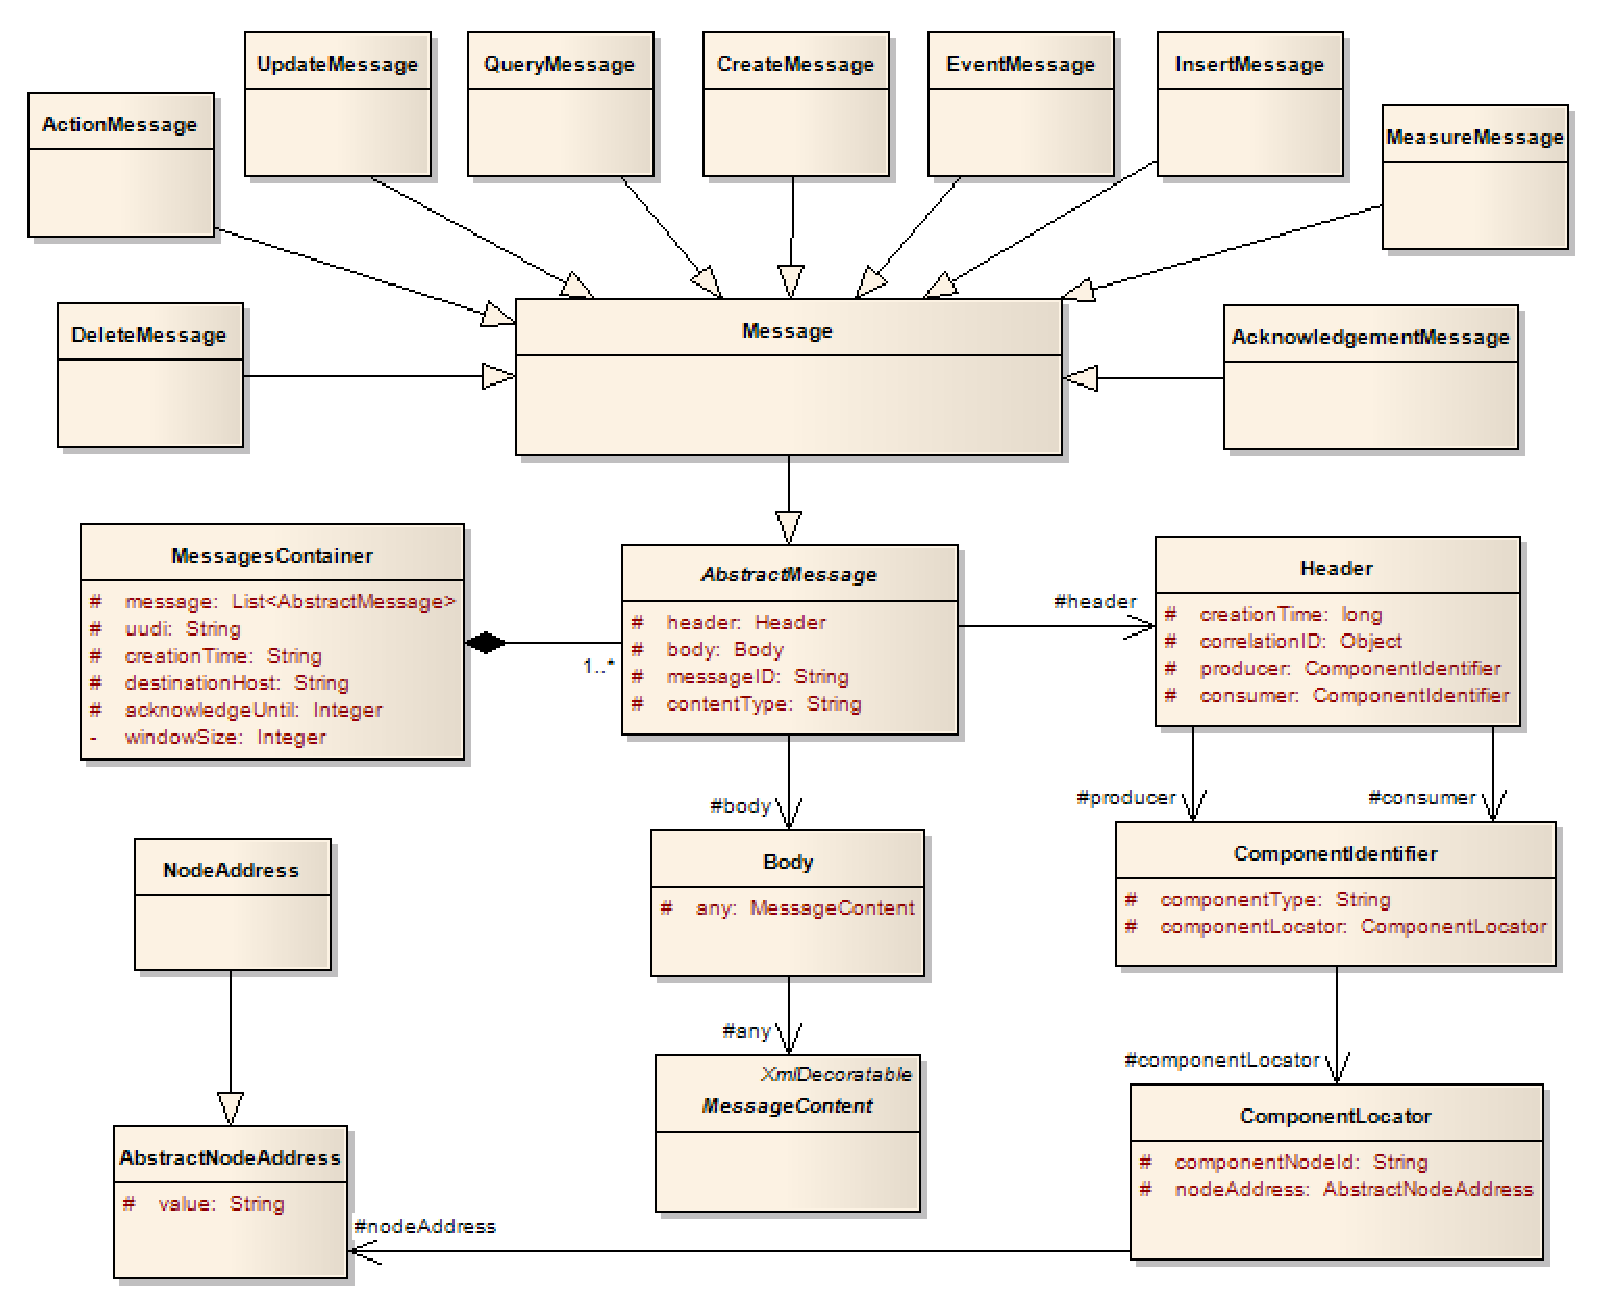
\includegraphics[scale=0.6]{../diagrams/DSP-Messages-Classes}
  \caption{The DSP Messages UML Class Diagram}
  \label{fig:DSP-Messages-Classes}
\end{figure}

Another use of the DSP Messages is during the DSP Platform activation process,
where bootstrap messages are used to configure each DSP component. In order to
send configuration parameters, the DSP Platform uses Update Messages using a
unique type of Message Content called DSP Properties, which is described in the
next section.

\section{Collected Sensor Data as the DSP Message Content}
\label{sec:dsp-payload-implementation}

As mentioned in the previsou section, a DSP Message can carry any data on its
body, also called the payload. In such a way, any data representation must
just extend from the Message Content abstract class as it is shown
\ref{fig:Sonde-MessageContainer-Class-Diagram}, as defines the data
representation of the YSI Sonde data.

\begin{figure}[!h]
  \centering
  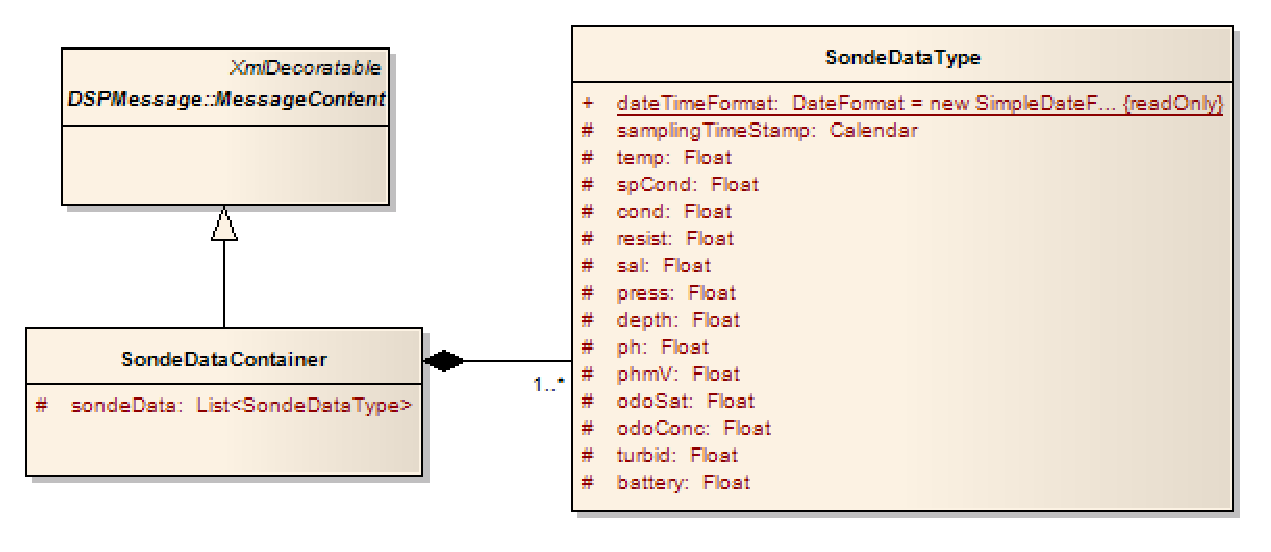
\includegraphics[scale=0.6]{../diagrams/Sonde-MessageContainer-Class-Diagram}
  \caption{The YSI Payload - Message Content UML Class Diagram}
  \label{fig:Sonde-MessageContainer-Class-Diagram}
\end{figure}

The properties measured from the YSI Sonde can be captured by the class
SondeDataType as a direct render of the measurements data depicted in table
\ref{tab:ysi-data-stream}. In addition to the regular data types, the class
also provides additional properties such as the attribute "samplingTimeStamp"
that carries the time when the data was collected from the YSI Sonde. However,
in order to capture a set of measurements at once, the SondeDataContainer
class used to carry a set of SondeDataType classes, as it is composed by one
or more instances of SondeDataType. In order to illustrate other examples,
consider the UML Class Diagram \cite{uml} of image
\ref{fig:Mouse-Actions--MessageContainer-Class-Diagram} as a payload of
observations made from a mouse over a screen, which captures the name of the
event, the button name and the x/y coordinates.

\begin{figure}[!h]
  \centering
  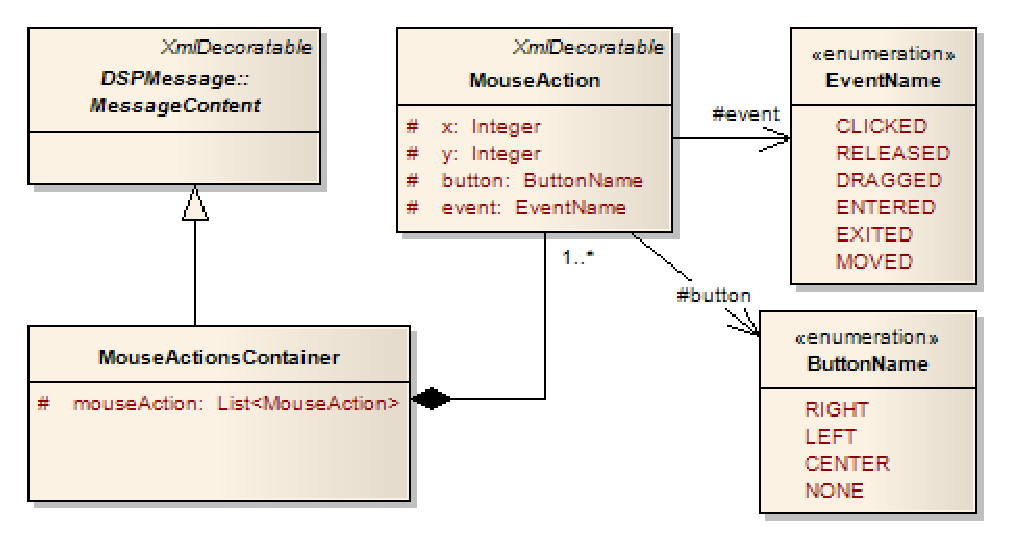
\includegraphics[scale=0.5]{../diagrams/Mouse-Actions--MessageContainer-Class-Diagram}
  \caption{The Mouse Actions Payload - Message Content UML Class Diagram}
  \label{fig:Mouse-Actions--MessageContainer-Class-Diagram}
\end{figure}

As described in the previous section, the DSP Platform uses DSP Update
Messages to configure internal components' initial configuration values. In
order to do so, the DSP Platform uses an instance of the DSP Properties, which
is composed of a list of initial DSP Property and their relating Values
instance depicted on the UML class diagram \cite{uml} of figure
\ref{fig:DSP-Property-Class-Diagram}. 

\begin{itemize}
  \item \textbf{Property Instance}: initial-rate
  \item \textbf{Value Instance}: 40
\end{itemize}

\begin{figure}[!t]
  \centering
  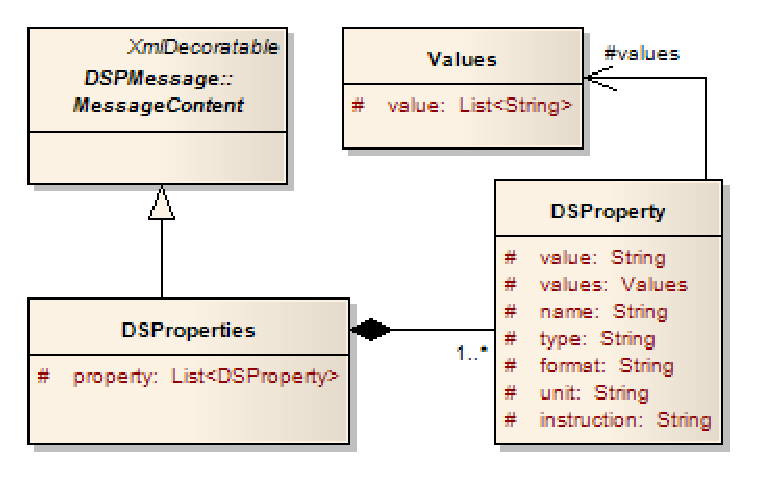
\includegraphics[scale=0.6]{../diagrams/DSP-Property-Class-Diagram}
  \caption{The DSP Property Payload - Message Content UML Class Diagram}
  \label{fig:DSP-Property-Class-Diagram}
\end{figure}

\subsection{DSP Platform Initialization Process}

All in all, the DSP Platform requires the knowledge of the aforementioned DSP
classes in order to initialize. The UML Sequence Diagram \cite{uml} in figure
\ref{fig:From-OSGi-DSP-Platform-Start-to-All-Components-Sequence-Diagram}
depicts the exact moments when the additional the plug-and-play DSP components
are installed and bootstrapped by the DSP Platform, as the UML State Diagram
\cite{uml} in Figure \ref{fig:DSPPlatform-Install-Usage-State-Diagram}
described.

\begin{itemize}
  \item \textbf{Start DSP Activator Gate}: after installing the Activator
  indicated by the DSP Bundle's MANIFEST.MF artifact, the OSGi Framework makes
  a call to the method Activator.start();
  \item \textbf{Bootstrap DSP Component Gate}: after the component has been
  initialized (by the call the method init() from the class ComponentManager),
  the DSP Component is ready to be bootstrapped, and the optional bootstrap
  message is delivered.
\end{itemize}

\begin{figure}[!b]
  \centering
  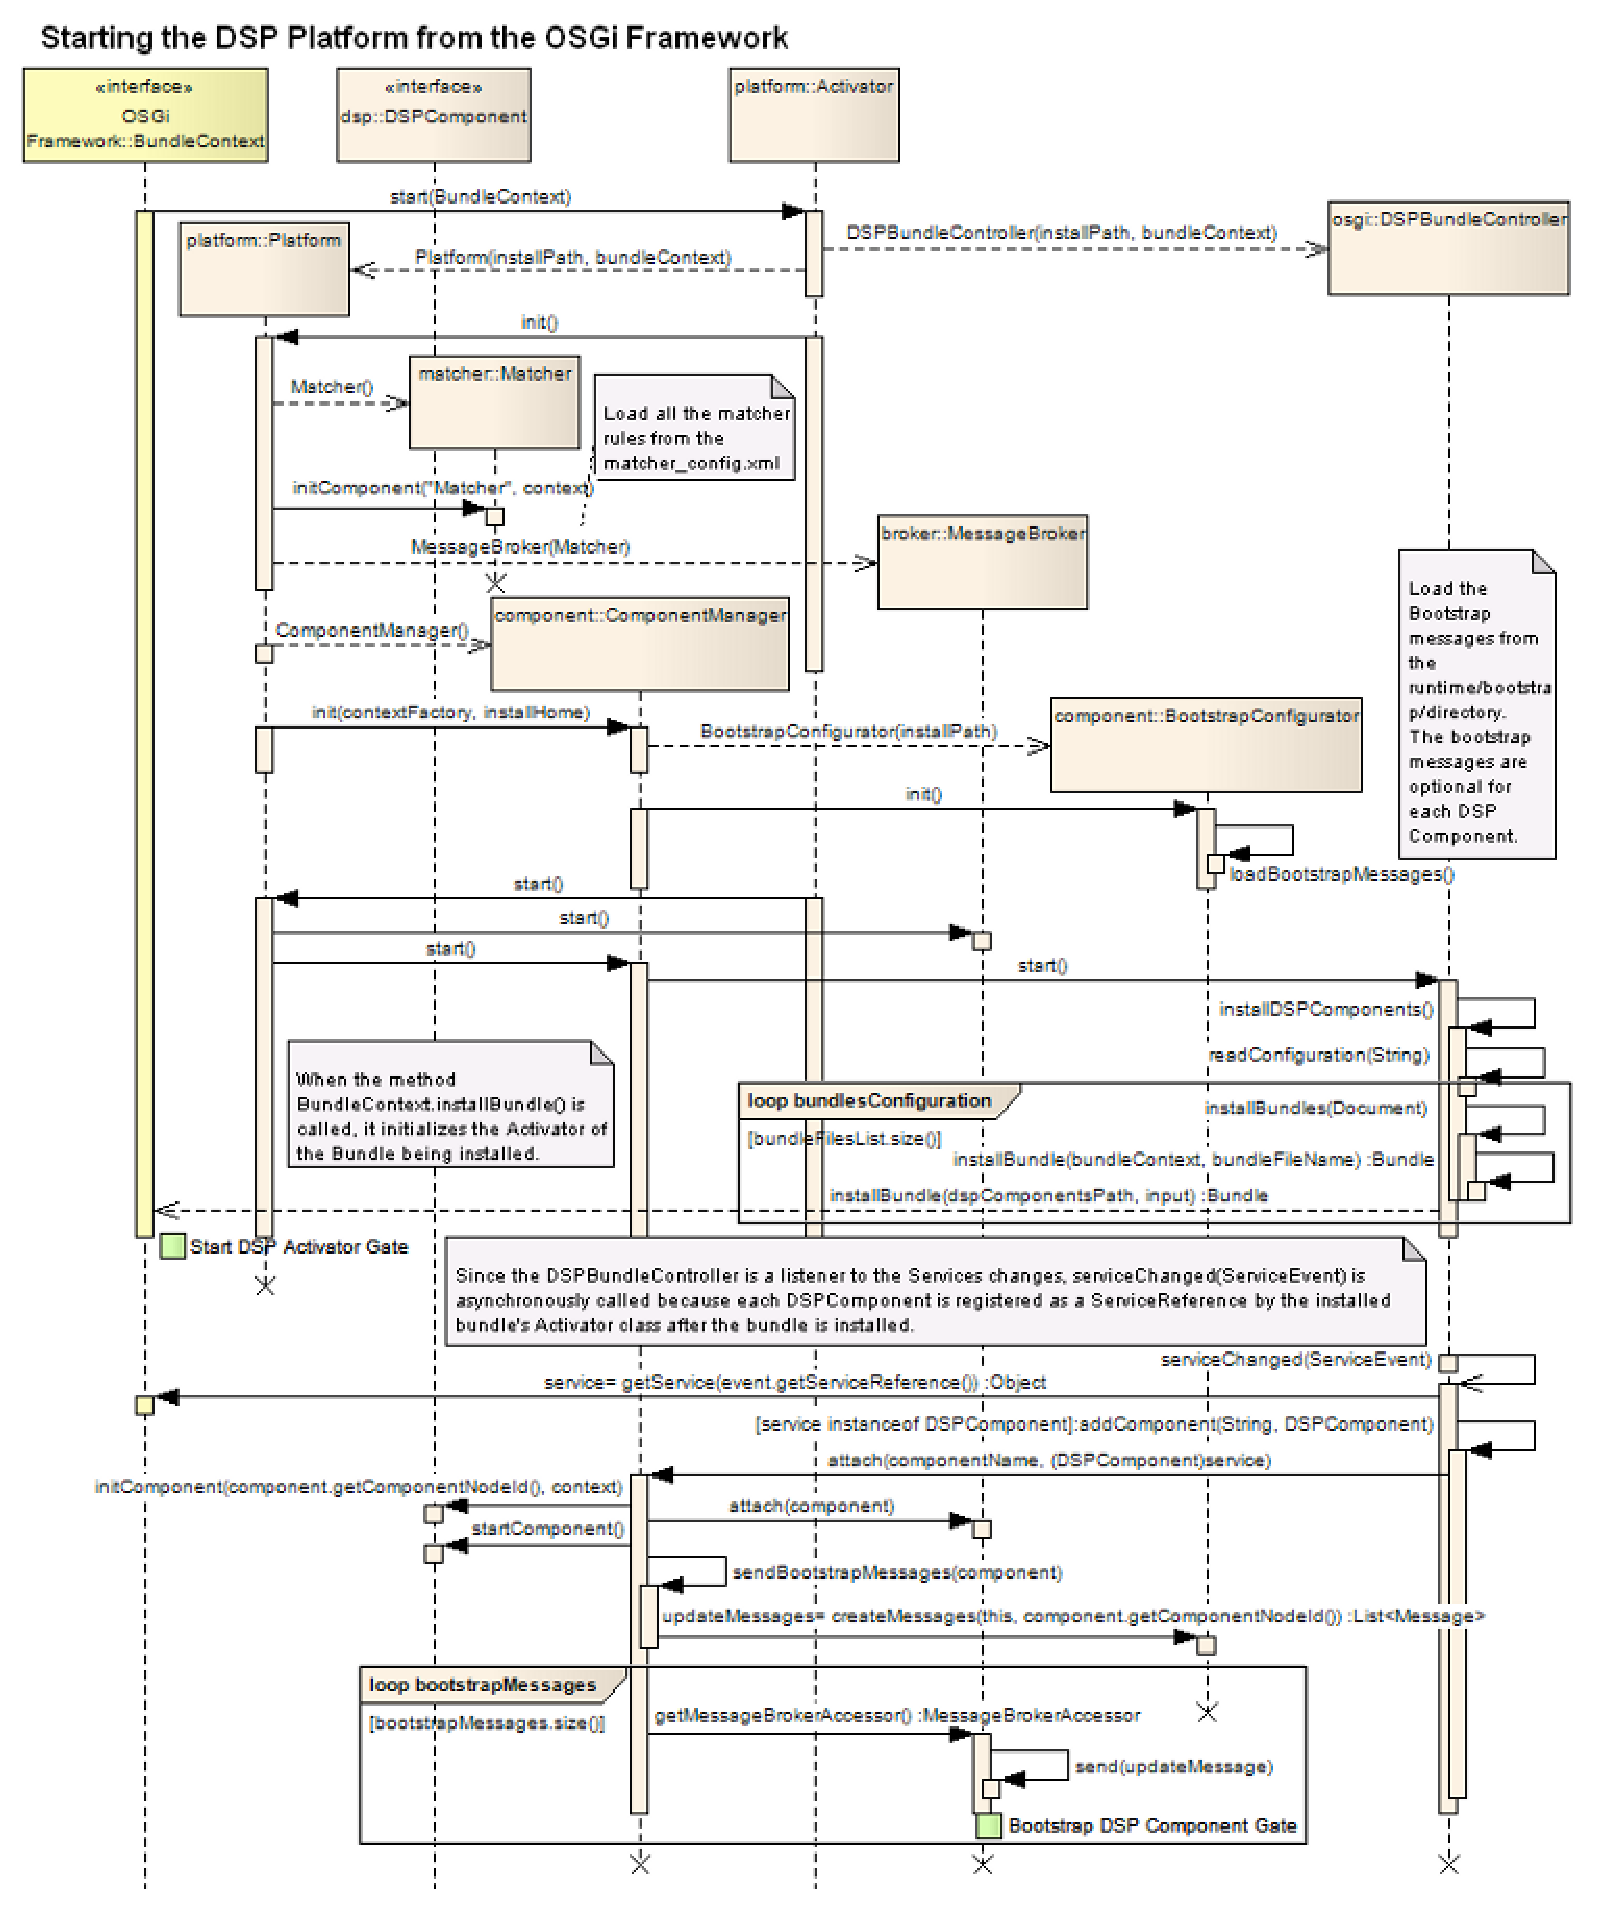
\includegraphics[scale=0.5]{../diagrams/From-OSGi-DSP-Platform-Start-to-All-Components-Sequence-Diagram}
  \caption{The DSP Platform Initialization UML Sequence Diagram}
  \label{fig:From-OSGi-DSP-Platform-Start-to-All-Components-Sequence-Diagram}
\end{figure}

\newpage

\subsection{Data Delivery Mechanism}

In general, when a DSP Component finishes preparing the DSP Messages Container,
it contacts an entity responsible for sending and proxying message to other
components. The DSP Broker acts like a mailman, receiving messages and
forwarding copies of it to other entities in the system, abstraction in which
is shown in Figure \ref{fig:DSP-Message-Broker-Abstraction}. In this way, the
DSP Broker receives a DSP Message and makes necessary deliveries to DSP
components that it has knowledge of.

\begin{figure}[!h]
  \centering
  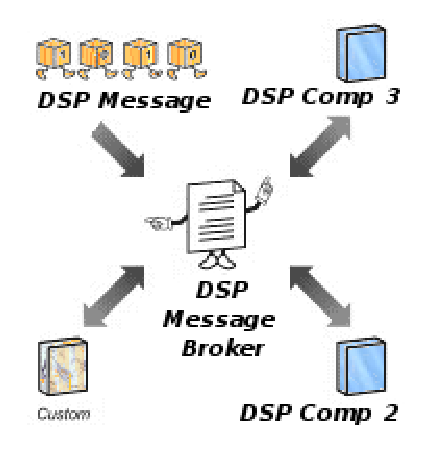
\includegraphics[scale=0.8]{../diagrams/DSP-Message-Broker-Abstraction}
  \caption{A DSP Message Broker Abstraction}
  \label{fig:DSP-Message-Broker-Abstraction}
\end{figure}

The use of messaging exchange paradigm is used in NetBEAMS because it decouples
the system by using messages take into account their structure to filter the
messages. In this way, the DSP Broker uses a filter component called DSP
Matcher, which provides a list of DSP Components that needs to receive a copy
of the DSP Message. It turns out that the DSP Matcher bases its decisions on
structured rules provided by the system administrator for an specific DSP
Platform instance. The UML Class diagram for the DSP Broker, Matcher and
particiaping classes is depicted in figure
\ref{fig:DSPBroker-Matcher-Class-Diagram}, and describes how the DSP Broker
implementation is tightly coupled with the DSP Matcher, as well as to the
lists of DSP Components sorted by name and type.

\begin{figure}[!b]
  \centering
  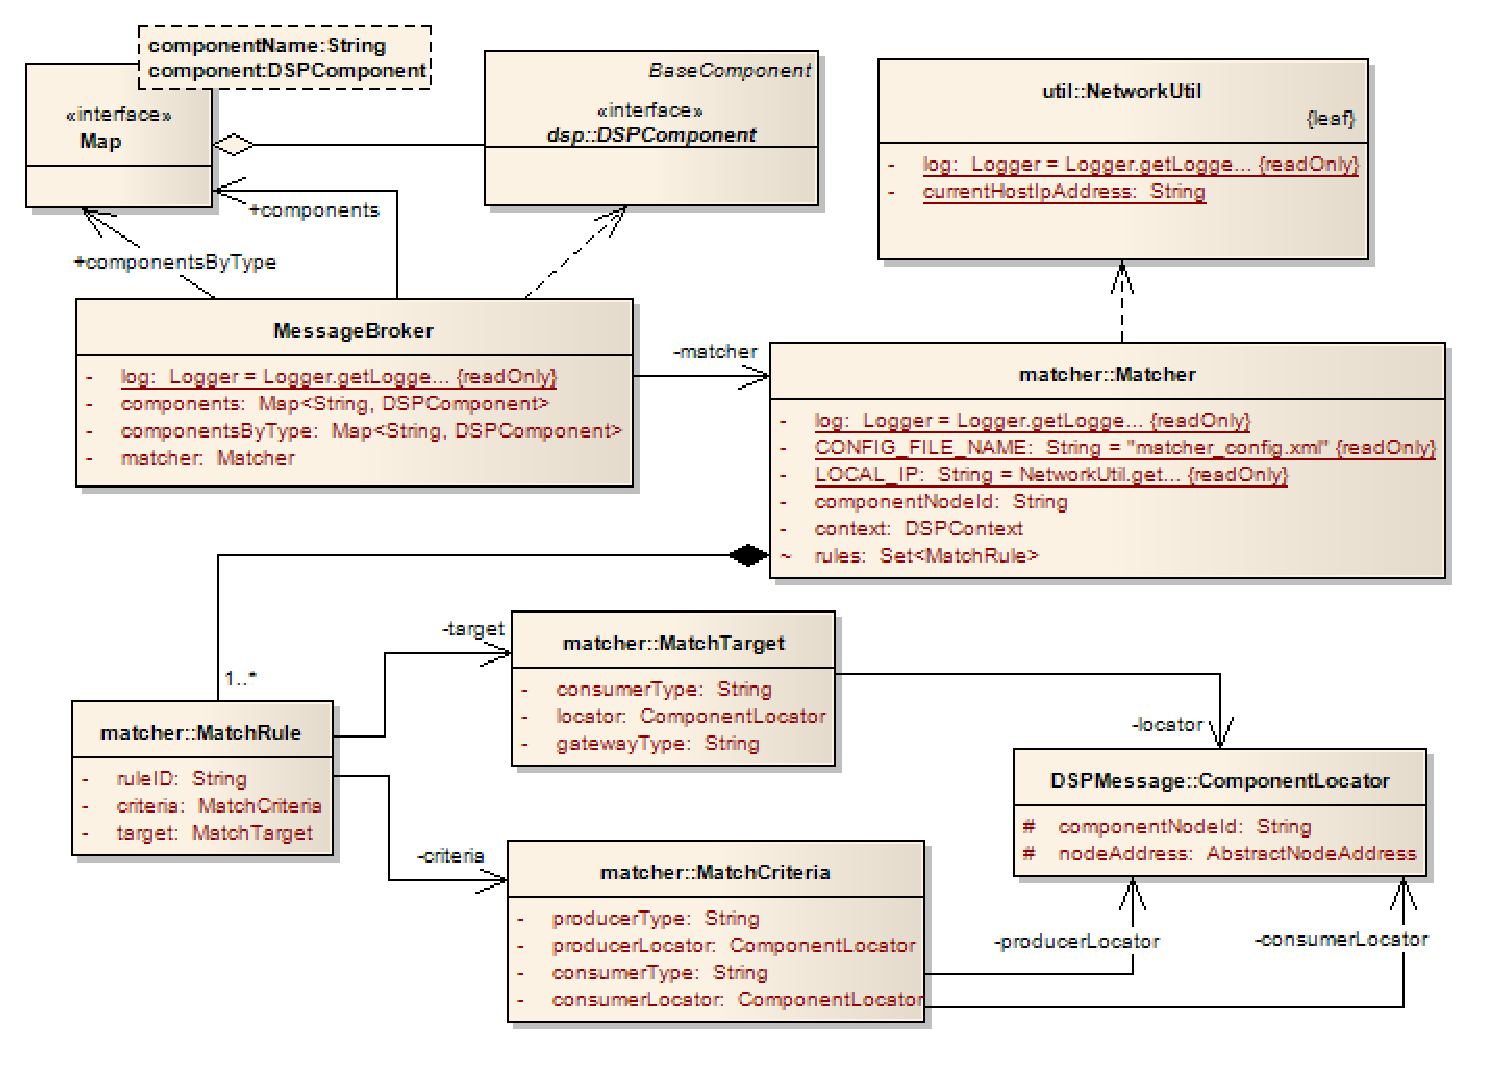
\includegraphics[scale=0.6]{../diagrams/DSPBroker-Matcher-Class-Diagram}
  \caption{The DSP Broker-Matcher UML Class Diagram}
  \label{fig:DSPBroker-Matcher-Class-Diagram}
\end{figure}

In general, the DSP Matcher is composed by a list of MatchRule, which contains
a reference to a MatchCriteria and a MatchTarget. The former identifies the
rule for matching a given DSP Message based on the producer and consumer's
message type and location, while the latter describes the DSP Component that
will receive the DSP Message, and if its delivery is done by means of a gateway
component. In this way, the DSP Matcher can be seen as a function, as depicted
in Table \ref{tab:matching-rule}, that takes a DSP Message as an input and
returns a list of DSP consumers, and the matching configuration artifact
provided by the administrator. See listing \ref{file:dsp-matcher-config.xml}) for details.

\begin{table}
    \caption{DSP Matcher Rule Algorithm to filter Data Consumer components to
    receive a given Message}
    \begin{center}
        \begin{tabular}{lr}
          \textit{Data Consumers ( DSP Message )} := \\ 
          Verify the DSP Message's Header + \\
          Verify the matcher rules, which contains the list of consumers for
          the given message
        \end{tabular}
    \end{center}
    \label{tab:matching-rule}
\end{table}

One example of such matching rule used by the DSP installed at the Gumstix can
be seen in listing \ref{file:dsp-matcher-config-gumstix.xml}. the Gumstix
system to configure the data delivery of the messages produced by the DSP
Component DSP Sonde Producer. It describes a list of maching rules that
reseambles a filtering system. This configuration contains 2 match rules: one
related to internal DSP Configuration and another for a remote destination.
The match criteria describes what the DSP Message Header properties must be,
while the match target is the destination of the message. One important
definition is the gateway Component Type, which defines the name of a remote
DSP Component that is capable of receiving a remote DSP Message.

Upon receiving all the matching rules and analyzing the DSP Message against
the rules, the DSP Broker selects a set of the running DSP components to receive
a copy of the DSP Message object in two different ways:

\begin{itemize}
  \item \textbf{In-memory local message delivery}: if the receiving DSP
  Component is located in the current local host, a deep copy of the instance
  of the DSP message is delivered;
    \begin{itemize}[label=\textbullet]
        \item IP Addresses are correctly resolved by using the Ethernet card in
        the device: localhost, 127.0.0.1, or the same IP Address for Producer
        and Receiver resolves into a local device. An example for such type of
        delivery can be seen in the match ruleID
        all messages sent to dsp manager of listing 
        \ref{file:dsp-matcher-config-gumstix.xml}.
    \end{itemize}
  \item \textbf{Serialized remote message delivery}: if the receiving DSP
  Component is located in a foreign/remote host, the message is serialized in a
  format defined by the transport protocol chosen the DSP Component responsible
  for the transport. The following section describes the existing DSP Data
  Transport component;     
  \begin{itemize}[label=\textbullet]
        \item IP Address from the Producer and Consumer are different, and are
        not resolved to be in the same host. An instance of such match rule can
        be seen in the match rule ID send-message-to-remote url dsp of the code
        snippet \ref{file:dsp-matcher-config-gumstix.xml}.
    \end{itemize}
\end{itemize}

\subsection{Sending DSP Messages through the Wire}
\label{sec:dsp-serialization}

In order to send messages through the wire, the DSP Platform uses two symmetric
components that serialize and deserialize DSP Messages to XML and back to Java
POJO, respectively, and vice-versa. Named DSP Wire Transport Client and DSP
Wire Transport Server \cite{netbeams2009}, these components use the HTTP
\cite{http} protocol to transport the serialized version of the DSP Messages.
Figure \ref{fig:DSP-to-DSP-Remote-Communication} depicts the scenario where a
DSP Sensor Node transmits a DSP Message through an HTTP POST request.

\begin{figure}[!b]
  \centering
  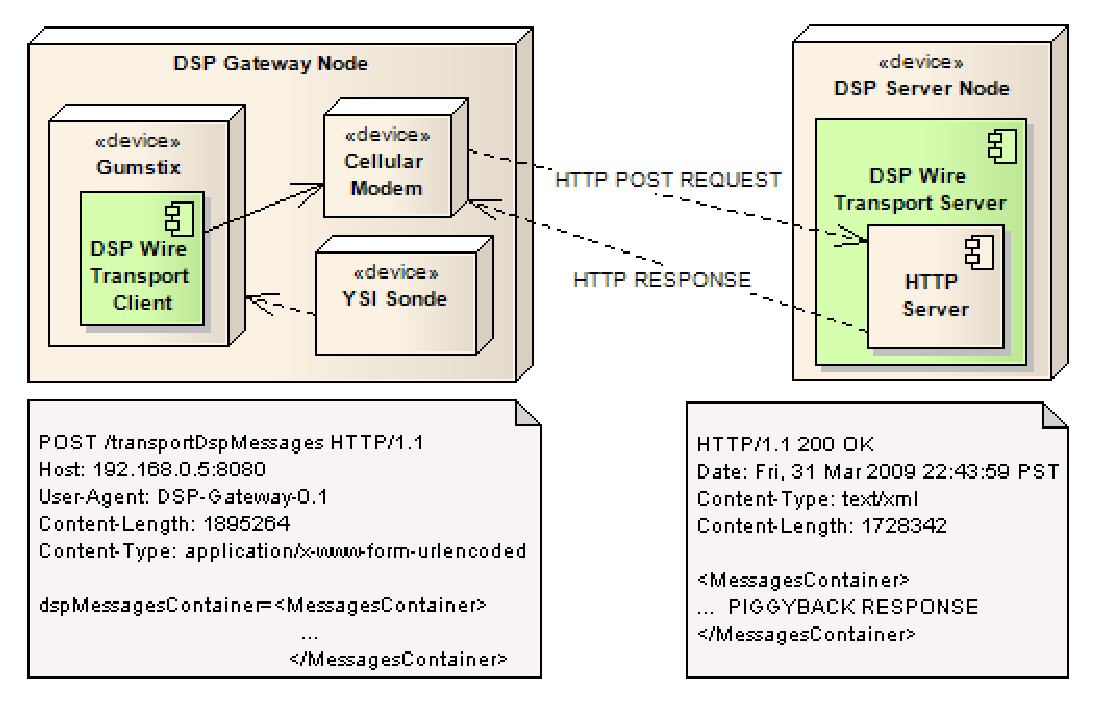
\includegraphics[scale=0.6]{../diagrams/DSP-to-DSP-Remote-Communication}
  \caption{The remote communication between two DSP Components using the HTTP
  Protocol}
  \label{fig:DSP-to-DSP-Remote-Communication}
\end{figure}

\begin{itemize}
  \item \textbf{DSP Wire Transport Client}: responsible for making HTTP POST
  Requests to the service provided by the DSP Wire Transport Server component.
  The body of the HTTP POST request contains a serialized version of an
  instance of a DSP MessagesContainer in XML format;
  \item \textbf{DSP Wire Transport Server}: exposes a Web Server listening to
  port 8080 that receives the HTTP POST request from the Client. Upon receiving
  the request, the server deserializes the DSP MessagesContainer back to the
  in-memory POJO and proceeds with the delivery to the DSP Broker. At this
  situation, the component packages acknowledgement messages and any queued
  message to the client and piggybacks \cite{xml-piggybacking} it to the HTTP
  response body.
\end{itemize}

As described by \cite{netbeams2009}, NetBEAMS is a single-hop sensor network
whose sensors transmits data from the sensors to the server. Upon receiving the
data stream, the DSP Wire Transport Server component desirializes the DSP
MessagesContainer and its enclosing DSP Messages back to a Java class instance
and delivers each of the DSP Messages to the DSP Broker, which delivers a
copy of the message to each DSP Component listed by the maching rule. 
%This
%process is depicted by the UML Sequence Diagram \cite{uml} in Figure \ref{fig:}

Whenever a DSP bundle producer is ready to transmit messages, they are added
into a DSP Messages Container (see UML Class Diagram in figure
\ref{fig:DSP-Messages-Classes}), which is serialized in XML to be transmitted.
Listing \ref{file:dsp-message-serialized-ysi} shows an instance of a DSP
MessagesContainer in serialized in XML, ready for transmission. In fact, the
listing is an example of the transmitted data collected from a sensor located
at the 192.168.0.103 to be transmitted to the host 192.168.0.106, and the
process of transmission in the server-side can be followed in figure
\ref{fig:From-DSPSondeComponent-to-DSPWireTransportClient-Sequence}.

\begin{figure}[!h]
  \centering
  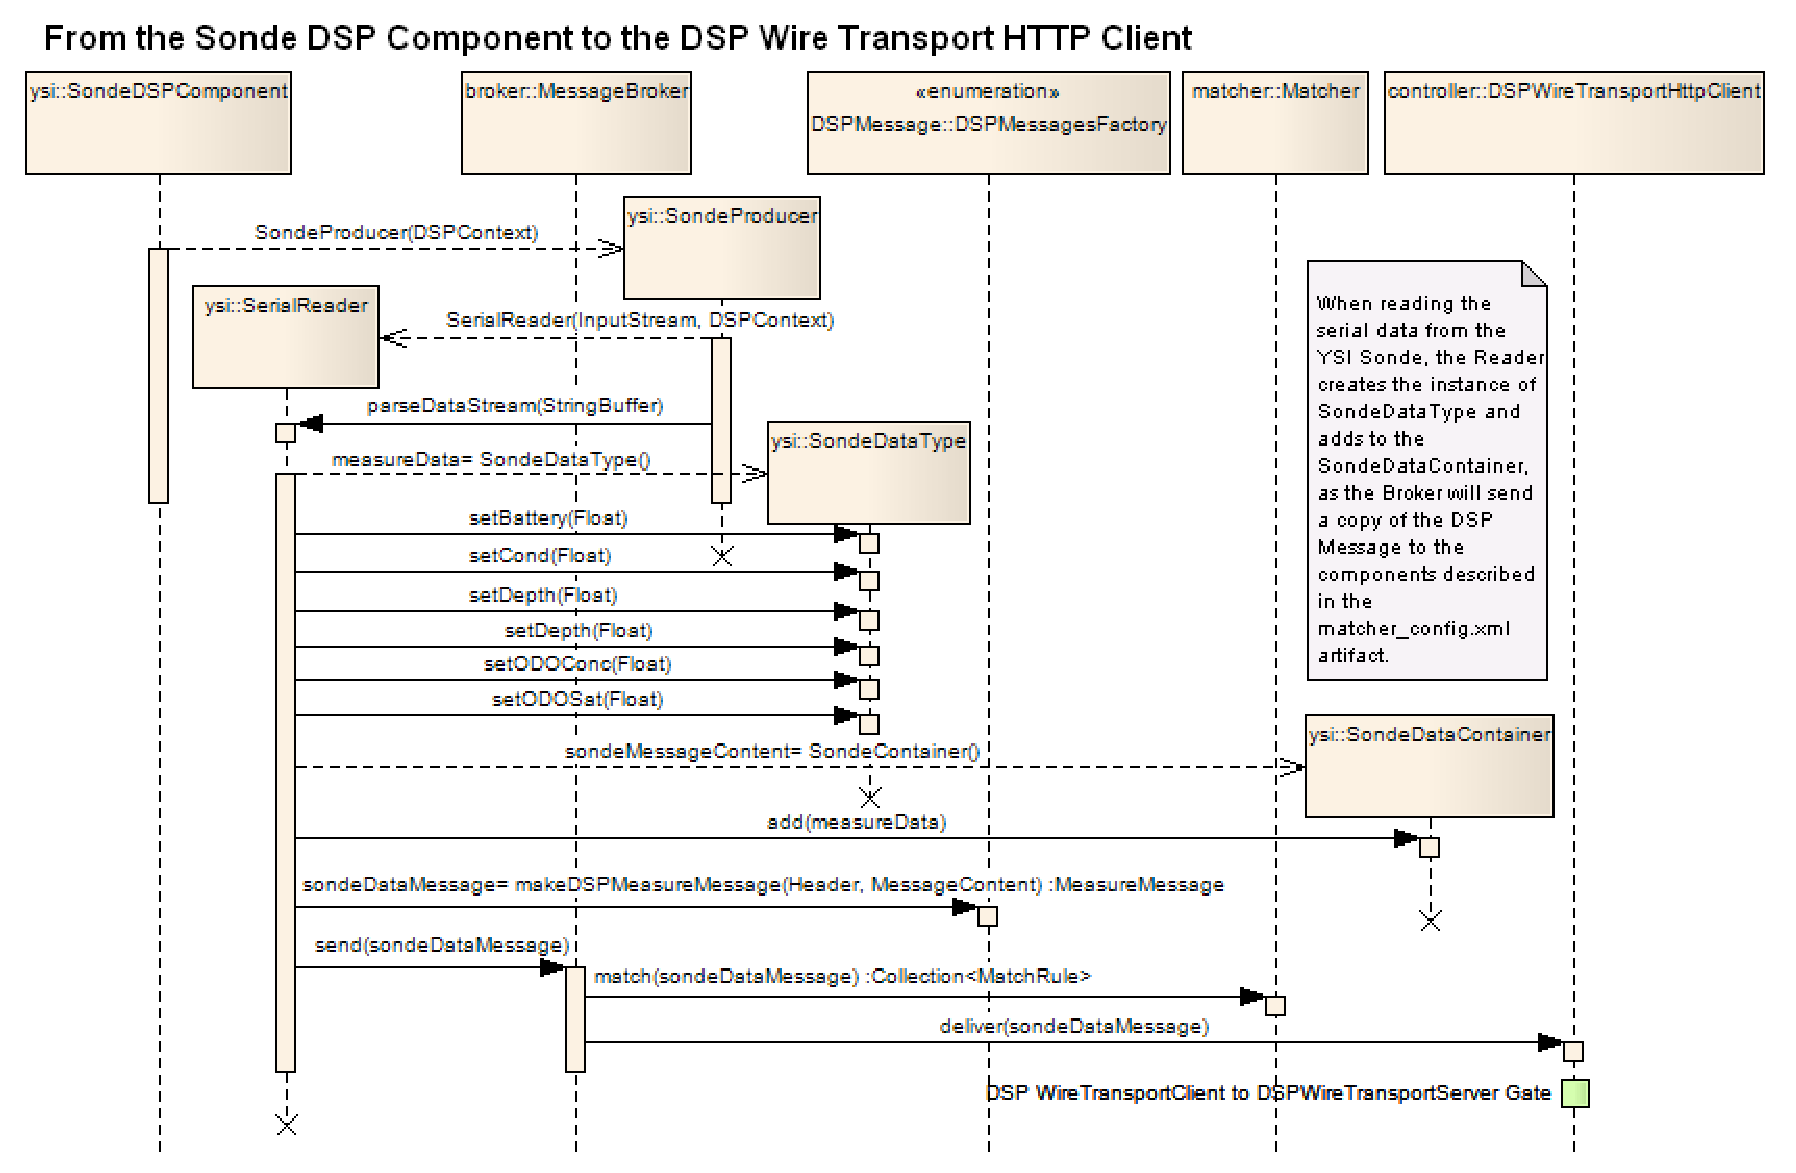
\includegraphics[scale=0.5]{../diagrams/From-DSPSondeComponent-to-DSPWireTransportClient-Sequence}
  \caption{The UML Sequence Diagram for the production of a YSI Message}
  \label{fig:From-DSPSondeComponent-to-DSPWireTransportClient-Sequence}
\end{figure}

The Sonde DSP Component is responsible for starting a worker thread called
SondeProducer, which is responsible for constantly read from the RS-232 serial
port by using an instance of the SerialReader class. This process depicts the
production of the data flow "flow 1" of figure
\ref{fig:netbeams-software-stack}, which is a collection of SondeDataType for
each of the measurement data read on a SondeDataContainer. As depicted in
figure \ref{fig:From-DSPSondeComponent-to-DSPWireTransportClient-Sequence}, it
first read the serial connection using the class SerialReader, which parses 
the data stream. After parsing the data, the reader creates an instance of the
class SondeDataType, the POJO responsible for carrying out the measurement
data. As described earlier, the data is added into the SondeDataContainer to
dispatched to the DSP Broker, whose responsibility is to get the list of DSP
Components that is setup to receive a copy of the DSP message (see previous
code snippet). As for the setup done for the Gumstix, the measurement message
is supposed to be sent to a remote destination of host 192.168.0.7. At this
point, the DSP Broker makes a decision to send the DSP Message to the default
gateway component DSPWireTransportClient.

After the message arrives in the DSPWireTransportClient, the message is
maintained in a temporary repository of outbound DSP Messages called
MessagesQueues after the message is hashed by the destination IP address and
the DSP Client sender using an instance of QueueMessageData. As shown in figure
\ref{fig:From-DSPWireTransport-Client-to-DSPWireTransportServer-Sequence}, the
DSP TransportSender is a worker thread that is started by the DSP Wire
Transport Client and is constantly transmits the data in the outbound queues
after a configurable rate. It makes a transport of the message and receives
the response, updates the state of the messages to transmitted, to finally
send the response messages to the DSP Message Broker.

\begin{figure}[!t]
  \centering
  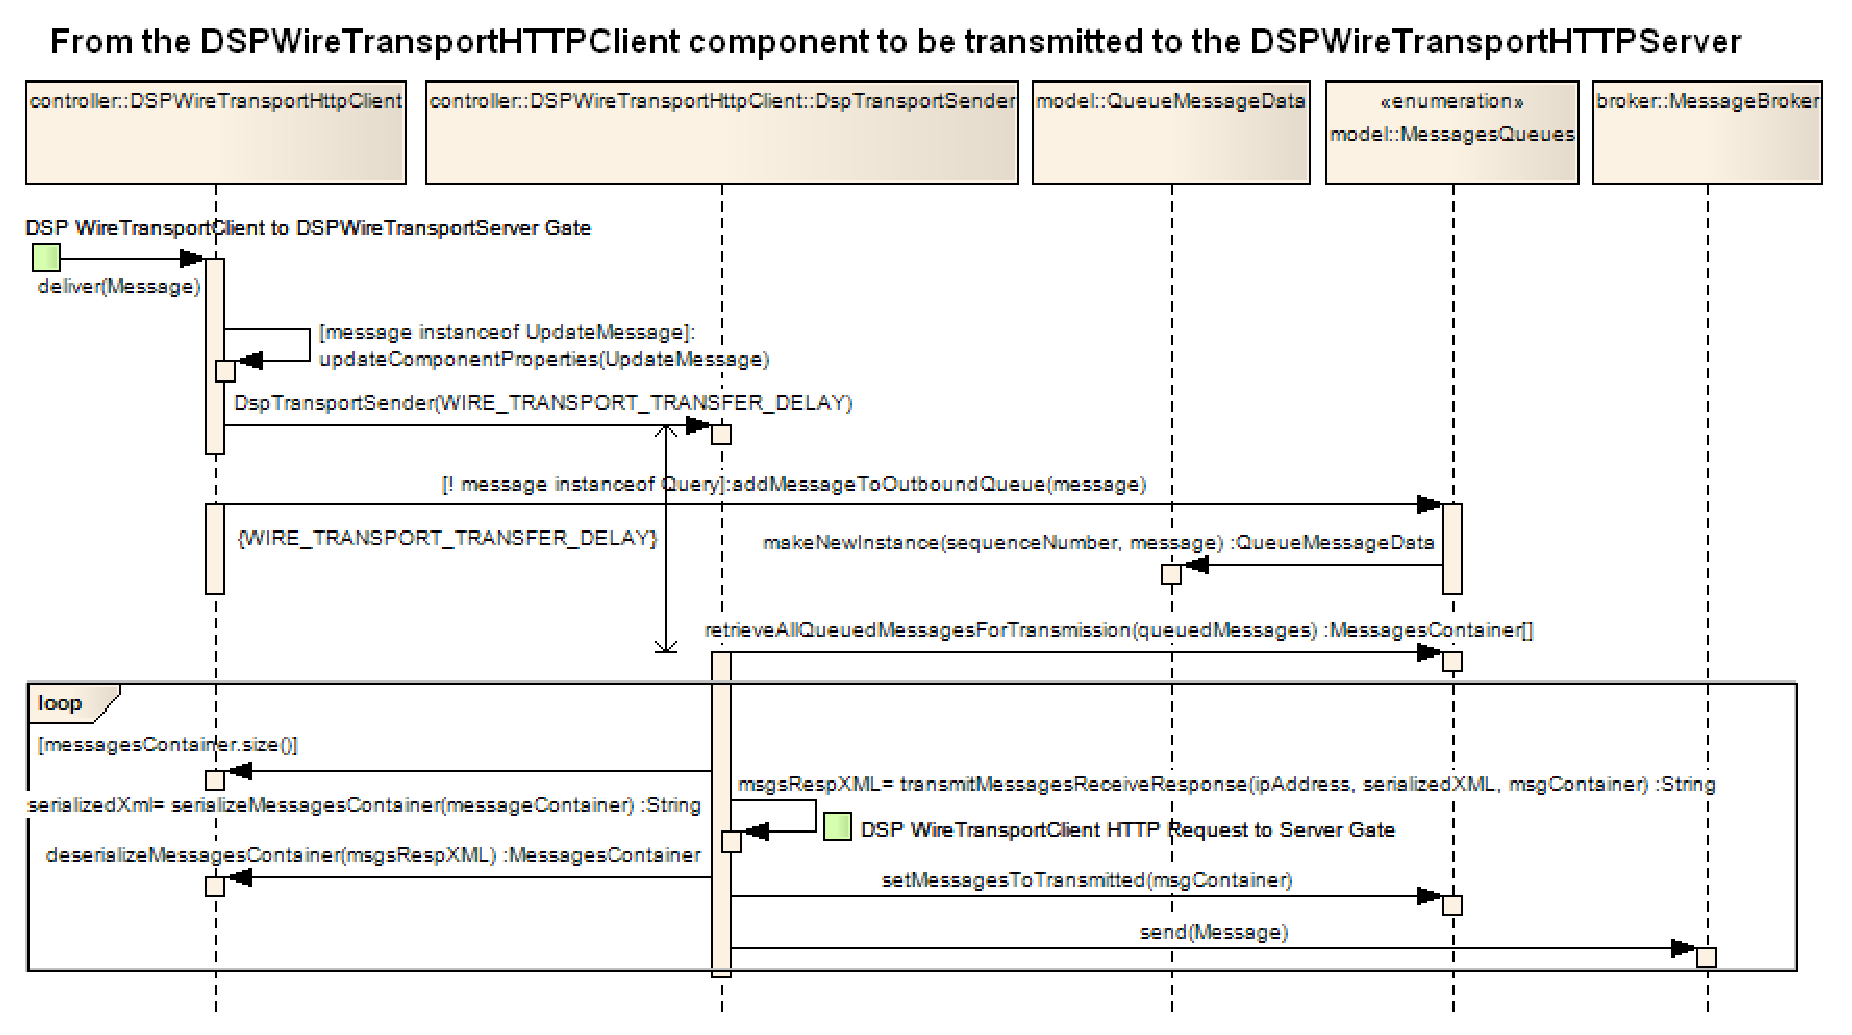
\includegraphics[scale=0.5]{../diagrams/From-DSPWireTransport-Client-to-DSPWireTransportServer-Sequence}
  \caption{The UML Sequence Diagram describing the Wire Transport Server
  receiving a DSP Message}
  \label{fig:From-DSPWireTransport-Client-to-DSPWireTransportServer-Sequence}
\end{figure}

While the DSPWireTransportClient makes an HTTP Request with the DSP Message,
the DSPWireTransportServer's servlet receives the request. It first
deserializes the MessagesContainer and delivers each of its messages to the DSP
Broker. At this point, the server verifies if there are messages in the
outbound queue that are addressed for the host that requested the messages
delivery. By using a technique called piggybacking, the server adds to the HTTP
Response a serialized version of the MessagesContainer with any DSP Messages.
In addition to any DSP Message, the server prepares and sends acknowledgement
messages back to the requesting host to the host.

\begin{figure}[!t]
  \centering
  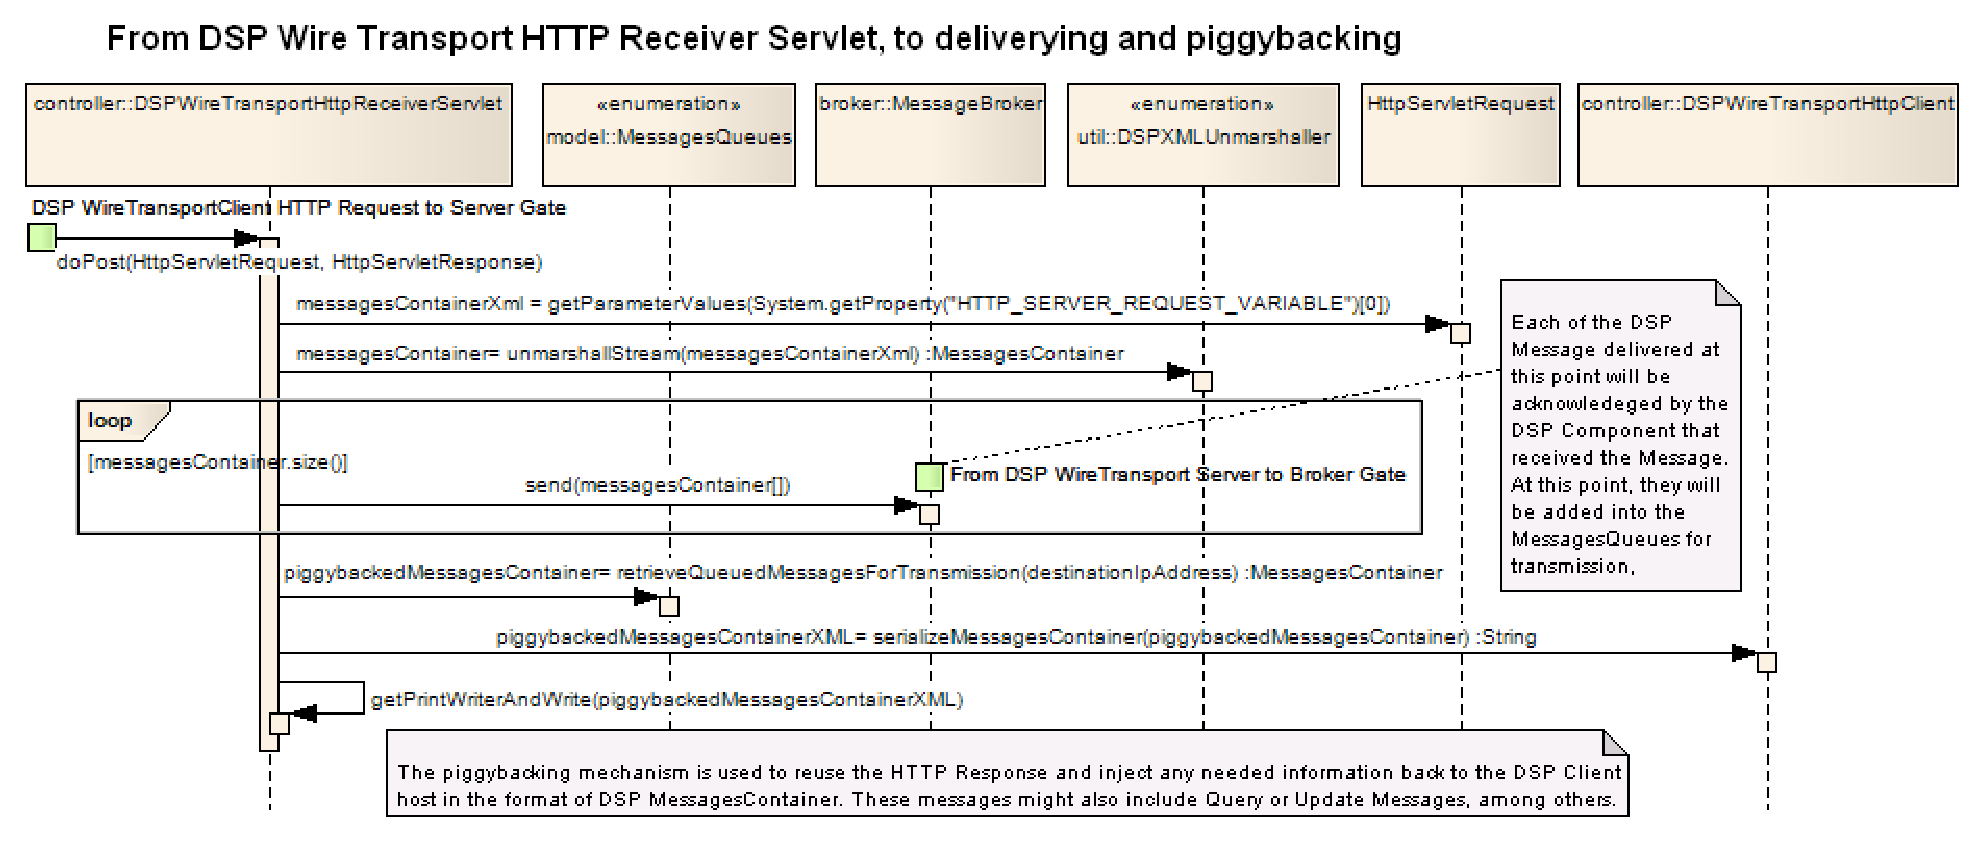
\includegraphics[scale=0.5]{../diagrams/From-DSPWireTransport-Server-To-DSP-Broker}
  \caption{The UML Sequence diagram describing the DSP
Message delivery on the server-side and the response}
  \label{fig:From-DSPWireTransport-Server-To-DSP-Broker}
\end{figure}

The gate "From DSP WireTransport Server to Broker Gate" defines the actual
delivery of the DSP Message to the DSP Broker. As this section is a tutorial
about the DSP Platform, the remaining steps will be explained on Section 3,
while showing the design and implementation of the component DSP Data
Persistence.

\section{DSP Data Persistence: Component Implementation}
\label{sec:dsp-data-persistence-implementation}

This section shows the implementation of the DSP Data Persistence, which
follows the specifications of the DSP Components in the previous chapter,
along with the setup of the mongoDB, the chosen database system that models
data in a type of key-value pair model. Moreover, this chapter also describes
the experiments conducted for the persistence.

The implementation of the DSP Data Persistence component, as well as the
implementation of the experiments, were developed and managed using the DSP a
reserved development branch at the Subversion \cite{subversion} repository
located at the Google Code website. In this way, anyone can checkout the entire
source-code from the branch
\textit{https://netbeams.googlecode.com/svn/branches/marcello/persistence},
as shown in Figure \ref{fig:dsp-data-persistence-dir}. In this way, the
recommended checkout branch directory will give the remaining directory
structure as summarized:

\begin{itemize}
  \item \textbf{NEBEAMS-DIR/}: the directories under the subdirectory
  ``persistence'';
  \item \textbf{DEV-VERSION}: the directory of the current development
  version for the DSP; That is, ``\textbf{NEBEAMS-DIR}/versions/v2/''
  \item \textbf{PERSISTENCE-DIR}: the directory of the DSP component, that is,
  ``\textbf{DEV-VERSION}/apps/osgi-intro-bundles/dsp/DSPDataPersistence''.
\end{itemize}

\begin{figure}[!b]
  \centering
  \includegraphics[scale=0.6]{../diagrams/dsp-data-persistence-dir}
  \caption{The DSP Data Persistence Directory Structure}
  \label{fig:dsp-data-persistence-dir}
\end{figure}

The DSP Platform defines its own run-time directory, which organizes the
artifacts used by the osgi-intro Framework, as well as the its own configuration
descriptor and matcher, as described in the previous section. 

\begin{itemize}
  \item \textbf{RUNTIME-DIR}: the main directory for the execution of the DSP
Platform, with all the necessary osgi-intro-related artifacts are placed, as shown in
Figure \ref{fig:dsp-runtime-dir}.
\end{itemize}

\begin{figure}[!t]
  \centering
  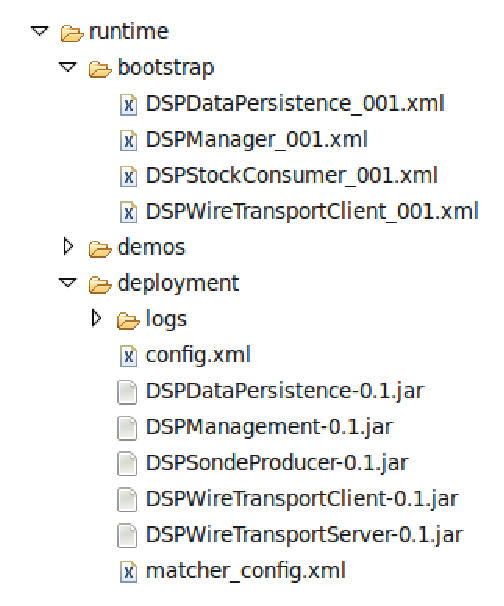
\includegraphics[scale=0.5]{../diagrams/dsp-runtime-dir}
  \caption{The DSP Data Persistence Directory Structure}
  \label{fig:dsp-runtime-dir}
\end{figure}

\section{DSP Platform Deployment Details}

As described in the previous chapter, the DSP Data Persistence Component was
implemented using the Java Programming language, on top of the osgi-intro Framework
API. This section describes the setup process of the implementation, as well as
the artifacts use during the implementation, which will be listed in the
appendix section.

The structure of the artifacts implemented for the DSP Data Persistence
Component follow the conventions of the NetBEAMS implementation, where the main
directory \textbf{PERSISTENCE-DIR}, depicted by Figure
\ref{fig:dsp-data-persistence-dir-checkedout}, holds each of the development
artifacts.

\begin{itemize}
  \item \textbf{DSPDataPersistence}: Main directory with the build.xml (Listing
  \ref{file:dsp-build.xml}) and other Eclipse-related artifacts. The other
  major directories are also listed:
  \item \textbf{META-INF}: this directory contains the descriptor file for
  the osgi-intro Framework, this this case the MANIFEST.MF;
  \item \textbf{src}: the main directory structure for the source-code
  implemented. Note that it follows the Java specification for packaging, and
  therefore, lists the package org.netbeams.dsp.persistence as the main
  package, including the layers controller, model and osgi-intro.
\end{itemize}

\begin{figure}[!h]
  \centering
  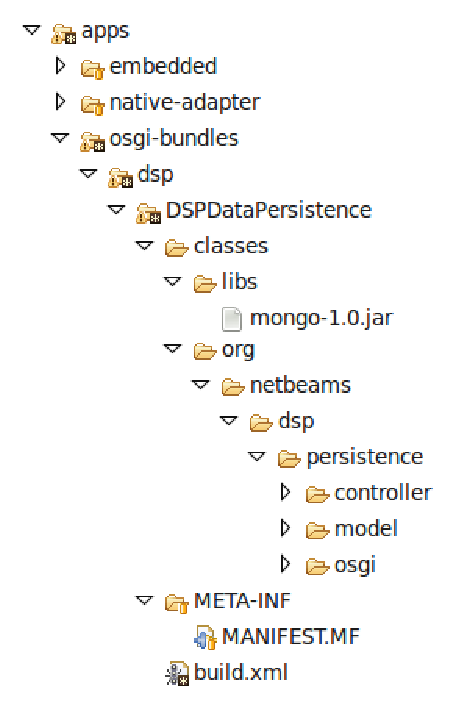
\includegraphics[scale=0.5]{../diagrams/dsp-data-persistence-dir-checkedout}
  \caption{The DSP Data Persistence Directory Structure}
  \label{fig:dsp-data-persistence-dir-checkedout}
\end{figure}

\subsection{osgi-intro Deployment Process}

Since each NetBEAMS component is managed by an osgi-intro component and its
infrastructure, this section describes the basic functionality of the osgi-intro
platform \cite{osgi-intro}, a framework was conceived to support modularity in
terms resources-limited environments such mobile devices and vehicles, but it
was first widely deployed on Eclipe IDE\footnote{Integrated Development
Environment}, because it promotes the use of reusable loosely-coupled modules
using the Java Programming Language \cite{java}. The most basic layer of the
osgi-intro Framework depicted in Figure \ref{fig:layering-osgi-intro} are as follows:

\begin{itemize}
  \item \textbf{Module Layer}: manages the osgi-intro bundles deployed on the osgi-intro
  Platform, providing the necessary "wiring" of the components. In other words,
  the modules, called osgi-intro Bundles, can export and/or import packages in the
  level of a Java Class managed by the osgi-intro Framework;
  \item \textbf{Service Layer}: resposible for the interoperability between 2
  or more bundles, enabling the bundles to register services offered by
  the its specification;
  \item \textbf{Execution Layer}: executes the bundles, managing and changing
  their life-cycle through the bundle execution.
\end{itemize}

\begin{figure}[!h]
  \centering
  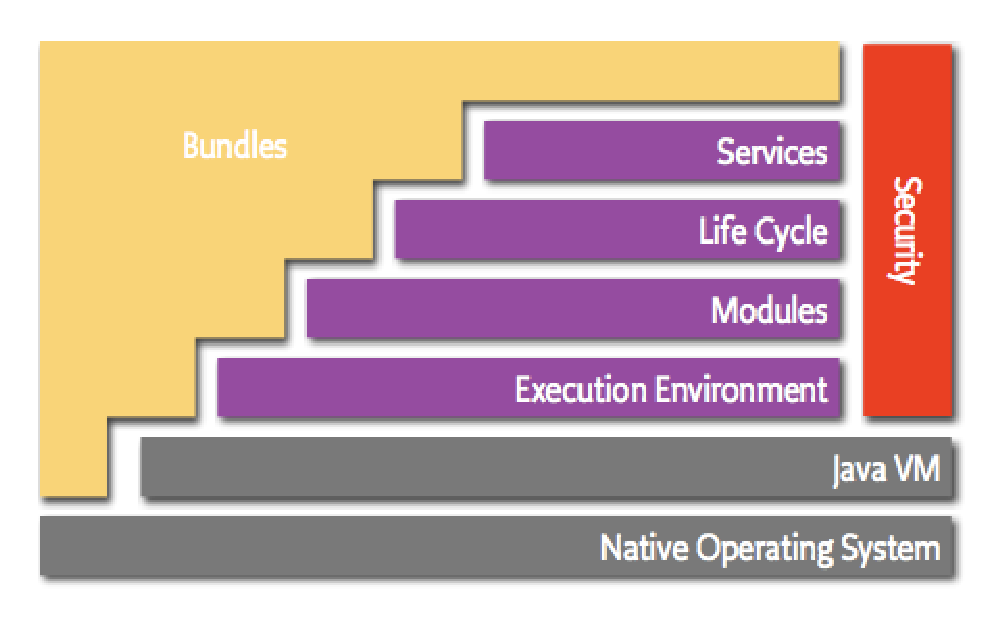
\includegraphics[scale=0.5]{../diagrams/layering-osgi}
  \caption{The osgi-intro Framework Layers}
  \label{fig:layering-osgi-intro}
\end{figure}

NetBEAMS uses the concept of the modularization through the use of the the
Producer-Consumer paradigm described in the previous section. Since the DSP
Components are essentially osgi-intro bundles, the interoperability between them are
given in the implementation and reuse existing bundles in the osgi-intro Framework
and the DSP Platform, described by an artifact called MANIFEST.MF as seen in
Listing \ref{file:osgi-intro-manifest}. In general, an osgi-intro bundle must
provide specifications that describes the module to be published into the osgi-intro
Framework. In this way, the main properties of the osgi-intro MANIFEST.MF artifact can
used by the DSP Data Persistence can be summarized as follows:

\begin{itemize}
  \item \textbf{Bundle-Activator}: The name of the instance of an osgi-intro Activator
  class, responsible to manage the bundle. The implemented class
  ``DataPersistenceActivator'' provides the activation mechanisms for the
  services provided by the DSP Data Persistence Component;
  \item \textbf{Bundle-ClassPath}: the necessary Java Jars list needed to run
  the bundle. It lists the mongoDB Java driver as one of the required
  dependencies deployed in the same package;
  \item \textbf{Import-Package}: the Java Packages needed by the DSP Data
  Persistence Component Bundle. These Java Packages must be provided by other
  DSP components, forcing the execution to be dependent on those package.
  They are provided through a ``Export-Package'' section in other osgi-intro
  bundles and, as it is shown in Listing \ref{file:osgi-intro-manifest}, they
  are from different packages.
\end{itemize}

Once the osgi-intro bundle is installed into the osgi-intro Platform, it will be managed by
the osgi-intro Execution layer and change the bundle state according to its
lify-cycle, as described in the previous chapter. Therefore, the packaging of
the osgi-intro source-code is done using a JAR\footnote{Java Archival Repository}
artifact specification \cite{java-tutorial}. In this way, the DSP Data
Platform osgi-intro bundle JAR is created by the Apache ANT build script
\cite{apache-ant} in Listing \ref{file:dsp-build.xml}. The task
``dsp-data-persistence.all'' compiles all the source-code created from the
design of the previous chapter and packages everything into the artifact
``DSPDataPersistence-x.x.jar'', where x.x is the version of the bundle. Figure
\ref{fig:dsp-runtime-dir} shows the DSP Data Persistence file under the
dirctory ``\textbf{RUNTIME-DIR}/deployment/''.

\subsection{Adding DSP Data Persistence into DSP Platform }

Once the new component was developed, the DSP Data Persistence component was
deployed by editing two main descriptors, as well as the optional bootstrap
message, as described in chapter 5:

\begin{itemize}
  \item \textbf{config.xml}: the DSP Data Persistence is added to the DSP
  Platform adding an entry for the component;
  \item \textbf{matcher\underline{ }config.xml}: the addition of the rules that
  filters the messages to the DSP Data Persistence;
  \item \textbf{DSPDataPersistence\underline{ }001.xml}: depicts the bootstrap
  message for the DSP Data Persistence Component, as shown in Listing 
  \ref{file:dsp-data-persistence-bootstrap.xml}.
\end{itemize}

The first configuration artifact enables NetBEAMS to initialize contain the
descriptor of the component, as shown in Listing \ref{file:dsp-config.xml}.
The component is added with the highest priority, since it contains
dependencies to other DSP Components. 
\subsection{Starting the DSP Platform}

Once the DSP Platform automatically installs all the components described by
the configuration descriptor, the container verifies the dependencies and
starts each of the DSP components of Figure \ref{fig:knopflerfish-execution},
the osgi-intro Framework container Knopflerfish \cite{knopflerfish}.

\begin{figure}[!t]
  \centering
  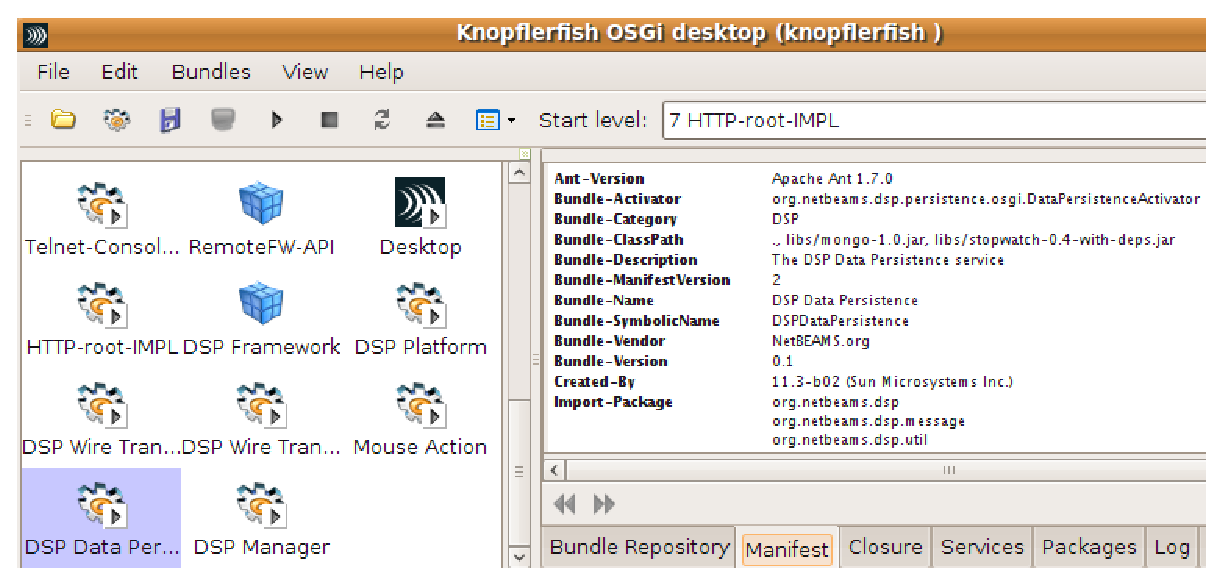
\includegraphics[scale=0.65]{../diagrams/knopflerfish-execution}
  \caption{The execution of the Knopflerfish Container}
  \label{fig:knopflerfish-execution}
\end{figure}

\section{mongoDB Deployment}
\label{sec:mongodb-deployment}

Given that Document-Oriented Model makes a good candidate persist sensors'
properties and the recently enumerated list technologies in the previous
article DSPDataPersistence, the open-source project called mongoDB was chosen
for the evaluation on our case study, the netBEAMS DSP Platform.

mongoDB supports storage based on collections of data, stored using BSON, a
binary representation the JSON data representation format, including dynamic
queries and indexing support. As it's stated in their web site, mongoDB
"bridges the gap between key/value stores (which are fast and highly scalable)
and traditional RDBMS systems (which are deep in functionality)".

\begin{itemize}
  \item mongoDB implements a document-oriented structure, which is similar to
  KVP;
  \item mongoDB is written in C++, and therefore, can is available in any major
  platform, as well as offers a broad range of API drivers written in different
  languages such as Java, Python, Perl and Ruby; 
  \item mongoDB is open-source, with good community support and availability
  through mailing lists, freenode IRC channel, and commercial support through
  10gen company; 
  \item mongoDB has support to distributed systems properties such as
  Master-Slave replication, and features like Database Shards with
  auto-sharding based on shard keys.
\end{itemize}

The artifacts of the mongoDB are located in the thirdparty directory of the
NetBEAMS resources. However, the build script from the DSP Data Persistence
component can be executed to produce the persistence directory
structure for NetBEAMS, as described in figure
\ref{fig:dsp-persistence-system-dir}.

\begin{figure}[!h]
  \centering
  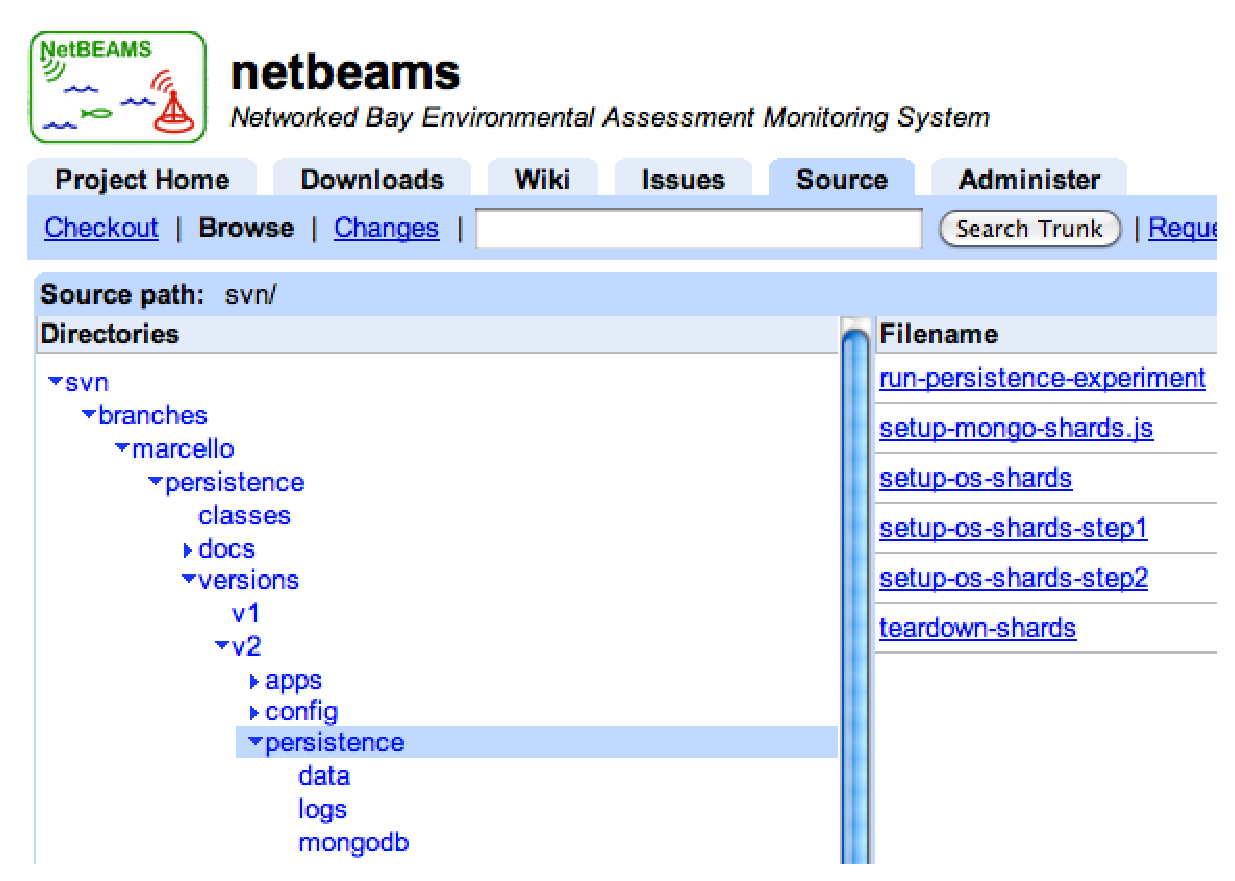
\includegraphics[scale=0.5]{../diagrams/dsp-persistence-system-dir}
  \caption{The osgi-intro Framework Layers}
  \label{fig:dsp-persistence-system-dir}
\end{figure}

\subsection{Document-Oriented Data Model}

An example of the data is as folows (using the JSON syntax). Listing
\ref{file:mongodb-ysi-data-format} follows the strategy described on Section X,
where the entity representation is denormalized, and each of the properties of
the sensor is repeated in each instance of the data. The fact and transaction
times are expressed in milliseconds. The data element contains the complete
structure of the originating sensor such as the IP address. The collection of
instances of this document represents the sensor data type.

\subsection{MongoDB Database Administration}

In order to start the database, just type ``mongod --dbpath DIRECTORY/

\section{Experiment Execution}
\label{sec:experiment-execution}

The experiments conducted using mongoDB can be summarized by the different
data access methods provided by the technology. Each subsection describes these
methods.

\subsection{Data Access Using Database Shell}
\label{sec:mongodb-user-experience}

The mongoDB client can be started by using the following command. Make sure you
have started the mongoDB server before executing the mongoDB client.

mongo netbeams | tee output\underline{ }number\underline{ }date.log

Here, the iterative mongo client shell offers users to verify and navigate on a
given database and its collections. This first section shows the connection of
the mongo client to the database netbeams. It also highlights the query for the
collections available. During the experiment, the SondeDataContainer?
collection was created as related to the type from the DSP Messages for the YSI
Sonde.

The shell references to the mongoDB system can be found at
http://www.mongodb.org/display/DOCS/dbshell+Reference 

\lstset{label=cmd:mongo,caption=Execution of mongo client}
\begin{lstlisting}
MongoDB shell version: 1.1.0-
url: netbeams
connecting to: netbeams
type "help" for help
> show collections
SondeDataContainer
system.indexes
>
> db.SondeDataContainer.count()
1000000
\end{lstlisting}

Then, the first verification of the data integrity is regarding the number of
elements created. Here, the first count() function on the collection returned
1000000.

An example about retrieving the first element of the collection can be done
using the findOne() function. It will return an element instance on the
JSONnotation.

\lstset{label=cmd:mongo-findone,caption=Querying the database: one item}
\begin{lstlisting}
> db.SondeDataContainer.findOne()
{
    "_id" : ObjectId("5d6f40078ec8074bba980900"),
    "message_id" : "020d82e1-18b2-4fe2-800c-a0f68e22ea86",
    "sensor" : {
        "ip_address" : "192.168.0.91",
        "location" : {
            "latitude" : 37.89155,
            "longitude" : -122.4464
        }
    },
    "time" : {
        "valid" : "Wed Nov 04 2009 02:30:12 GMT-0800 (PST)",
        "transaction" : "Sat Nov 21 2009 03:01:33 GMT-0800 (PST)"
    },
    "observation" : {
        "WaterTemperature" : 88.58,
        "SpecificConductivity" : 180.5,
        "Conductivity" : 167.3,
        "Resistivity" : 491.89,
        "Salinity" : 0.06,
        "Pressure" : 1.109,
        "Depth" : 2.642,
        "pH" : 7.11,
        "pHmV" : -42.9,
        "Turbidity" : 0.2,
        "ODOSaturation" : 72.4,
        "ODO" : 10.85,
        "Battery" : 2.7
    }
}
\end{lstlisting}

The query based on attributes can be done using the "dot" notation, as you
navigate through the JSON documents. Additionally, you can use the functions as
aggregated on the result of others. The example in listing
\ref{cmd:mongo-find-list} counts the number of documents with the key
"data.ph" equals to "5.64".

\lstset{label=cmd:mongo-find-list,caption=Execution of mongo client}
\begin{lstlisting}
> db.SondeDataContainer.find({"data.ph":5.64)}).count()
1226
\end{lstlisting}

The following example is the output of the first 2 documents from the same
previous query using the limit() function, as shown in figure
\ref{cmd:mongo-find-limit}.

\lstset{label=cmd:mongo-find-limit,caption=Query Element with specific
projection limiting the result set size}
\begin{lstlisting}
> db.SondeDataContainer.find({"data.ph":5.64}).limit(2)
{"_id" :  ObjectId( "d36f4007b7e7ac4a03c60000")  , "sensor_ip_address" : "192.168.0.136" , "message_id" : "7b6624d6-0ca1-4cba-a343-f166e88da73b"
, "transaction_time" : 1252845473412 , "fact_time" : 1252845346000 , "data" : {"temperature" : "45.01" , "sp_condition" : "37.6" ,
"condition" : "145.8" , "resistence" : "159.77" , "salinitude" : "0.0" , "pressure" : "0.391" , "depth" : "0.46" , "ph" : "5.64" ,
"pH_mv" : "-62.1" , "odo_sat" : "89.7" , "odo_condition" : "59.34" , "turbidity" : "0.0" , "battery" : "9.4"}}
{"_id" :  ObjectId( "d36f4007b7e7ac4a1fc80000")  , "sensor_ip_address" : "192.168.0.136" , "message_id" : "7b6624d6-0ca1-4cba-a343-f166e88da73b" ,
"transaction_time" : 1252845473412 , "fact_time" : 1252845346000 , "data" : {"temperature" : "46.71" , "sp_condition" : "60.8" ,
"condition" : "160.6" , "resistence" : "1399.4" , "salinitude" : "0.01" , "pressure" : "1.057" , "depth" : "2.485" , "ph" : "5.64" ,
"pH_mv" : "-16.3" , "odo_sat" : "58.8" , "odo_condition" : "19.29" , "turbidity" : "0.2" , "battery" : "9.2"}}
>
\end{lstlisting}

Other logs are located at
http://code.google.com/p/netbeams/downloads/list

\subsection{Data Access Using APIs}

The mongoDB server offers different drivers to access the data, as well as the
Web Services.

\begin{itemize}
  \item The Java tutorial on the drivers is located at
    http://www.mongodb.org/display/DOCS/Java+Tutorial. The driver is located on
    the NETBEAMS/versions/v2/thirdparty/mongodb directory;  
  \item The REST API can be called from any HTTP client. At the time of the
  editing, this feature is still under alpha version. Check the documentation
  athttp://www.mongodb.org/display/DOCS/Http+Interface for details 
\end{itemize}

The following HTTP GET Request method returns the first 5 documents in the collection:
http://127.0.0.1:28017/netbeams/SondeDataContainer/?limit=-5, as shown in
listing \ref{cmd:mongo-rest-request}.

\lstset{label=cmd:mongo-rest-request,caption=REST HTTP GET Request Example}
\begin{lstlisting}
http://192.168.1.2:28017/netbeams/SondeDataContainer/?limit=-3&filter_observation.Conductivity=104.5

HTTP/1.0 200 OK
x-action:
x-ns: netbeams.SondeDataContainer
Content-Type: text/plain;charset=utf-8

{
  "offset" : 0,
  "rows": [
    { "_id" : { "$oid" : "616f400784ba194bc2dee200" }, "message_id" : "c76a9898-1eee-4463-bf5d-d40a7a8af6e3", "sensor" : { "ip_address" : "192.168.0.60", "location" : { "latitude" : 37.89155, "longitude" : -122.4464 } }, "time" : { "valid" : { "$date" : 1261229067000 }, "transaction" : { "$date" : 1259977271704 } }, "observation" : { "WaterTemperature" : 51.29, "SpecificConductivity" : 110.7, "Conductivity" : 104.5, "Resistivity" : 1710.07, "Salinity" : 0.01, "Pressure" : 1.094, "Depth" : 1.808, "pH" : 3.04, "pHmV" : -46.4, "Turbidity" : 0.2, "ODOSaturation" : 59, "ODO" : 10.66, "Battery" : 7.1 } } ,
    { "_id" : { "$oid" : "616f400789ba194bdbe2e200" }, "message_id" : "2eb3f5ca-7a30-4b5d-8d16-c3e80a7b1b7a", "sensor" : { "ip_address" : "192.168.0.24", "location" : { "latitude" : 37.89155, "longitude" : -122.4464 } }, "time" : { "valid" : { "$date" : 1261740924000 }, "transaction" : { "$date" : 1259977271704 } }, "observation" : { "WaterTemperature" : 10.98, "SpecificConductivity" : 100.9, "Conductivity" : 104.5, "Resistivity" : 5448.21, "Salinity" : 0.08, "Pressure" : 1.152, "Depth" : 1.289, "pH" : 3.09, "pHmV" : -0.4, "Turbidity" : 0.1, "ODOSaturation" : 72.2, "ODO" : 59.65, "Battery" : 6.3 } } ,
    { "_id" : { "$oid" : "616f400789ba194b13e5e200" }, "message_id" : "a7804d0a-44a8-4bd9-a9c7-51db84e91f08", "sensor" : { "ip_address" : "192.168.0.236", "location" : { "latitude" : 37.89155, "longitude" : -122.4464 } }, "time" : { "valid" : { "$date" : 1260969259000 }, "transaction" : { "$date" : 1259977271704 } }, "observation" : { "WaterTemperature" : 7.97, "SpecificConductivity" : 119.1, "Conductivity" : 104.5, "Resistivity" : 1971.59, "Salinity" : 0.05, "Pressure" : 1.516, "Depth" : 2.187, "pH" : 3.11, "pHmV" : -77.59999999999999, "Turbidity" : 0.2, "ODOSaturation" : 82.90000000000001, "ODO" : 41.99, "Battery" : 0.1 } }
  "total_rows" : 3 ,
  "query" : {} ,
  "millis" : 0
}
\end{lstlisting}

Data visualisation tools for mongoDB is slowly being developed by open-source
developers. The next picture shows the database "netbeams" and the collection
"SondeDataContainer  ?" being rendered by futon4mongodb, one of the
open-source tools developed to visualise mongoDB data.

\subsection{Visualizing Data on The Browser}

Futon4Mongo is an open-source software adapted from CouchDB \cite{couchdb}.
First, the collections list is shown. Figure
\ref{fig:view-collections-instance-browser-futondb} shows one single collection
for the YSI data containing 1 million objects.

\begin{figure}[h]
  \centering
  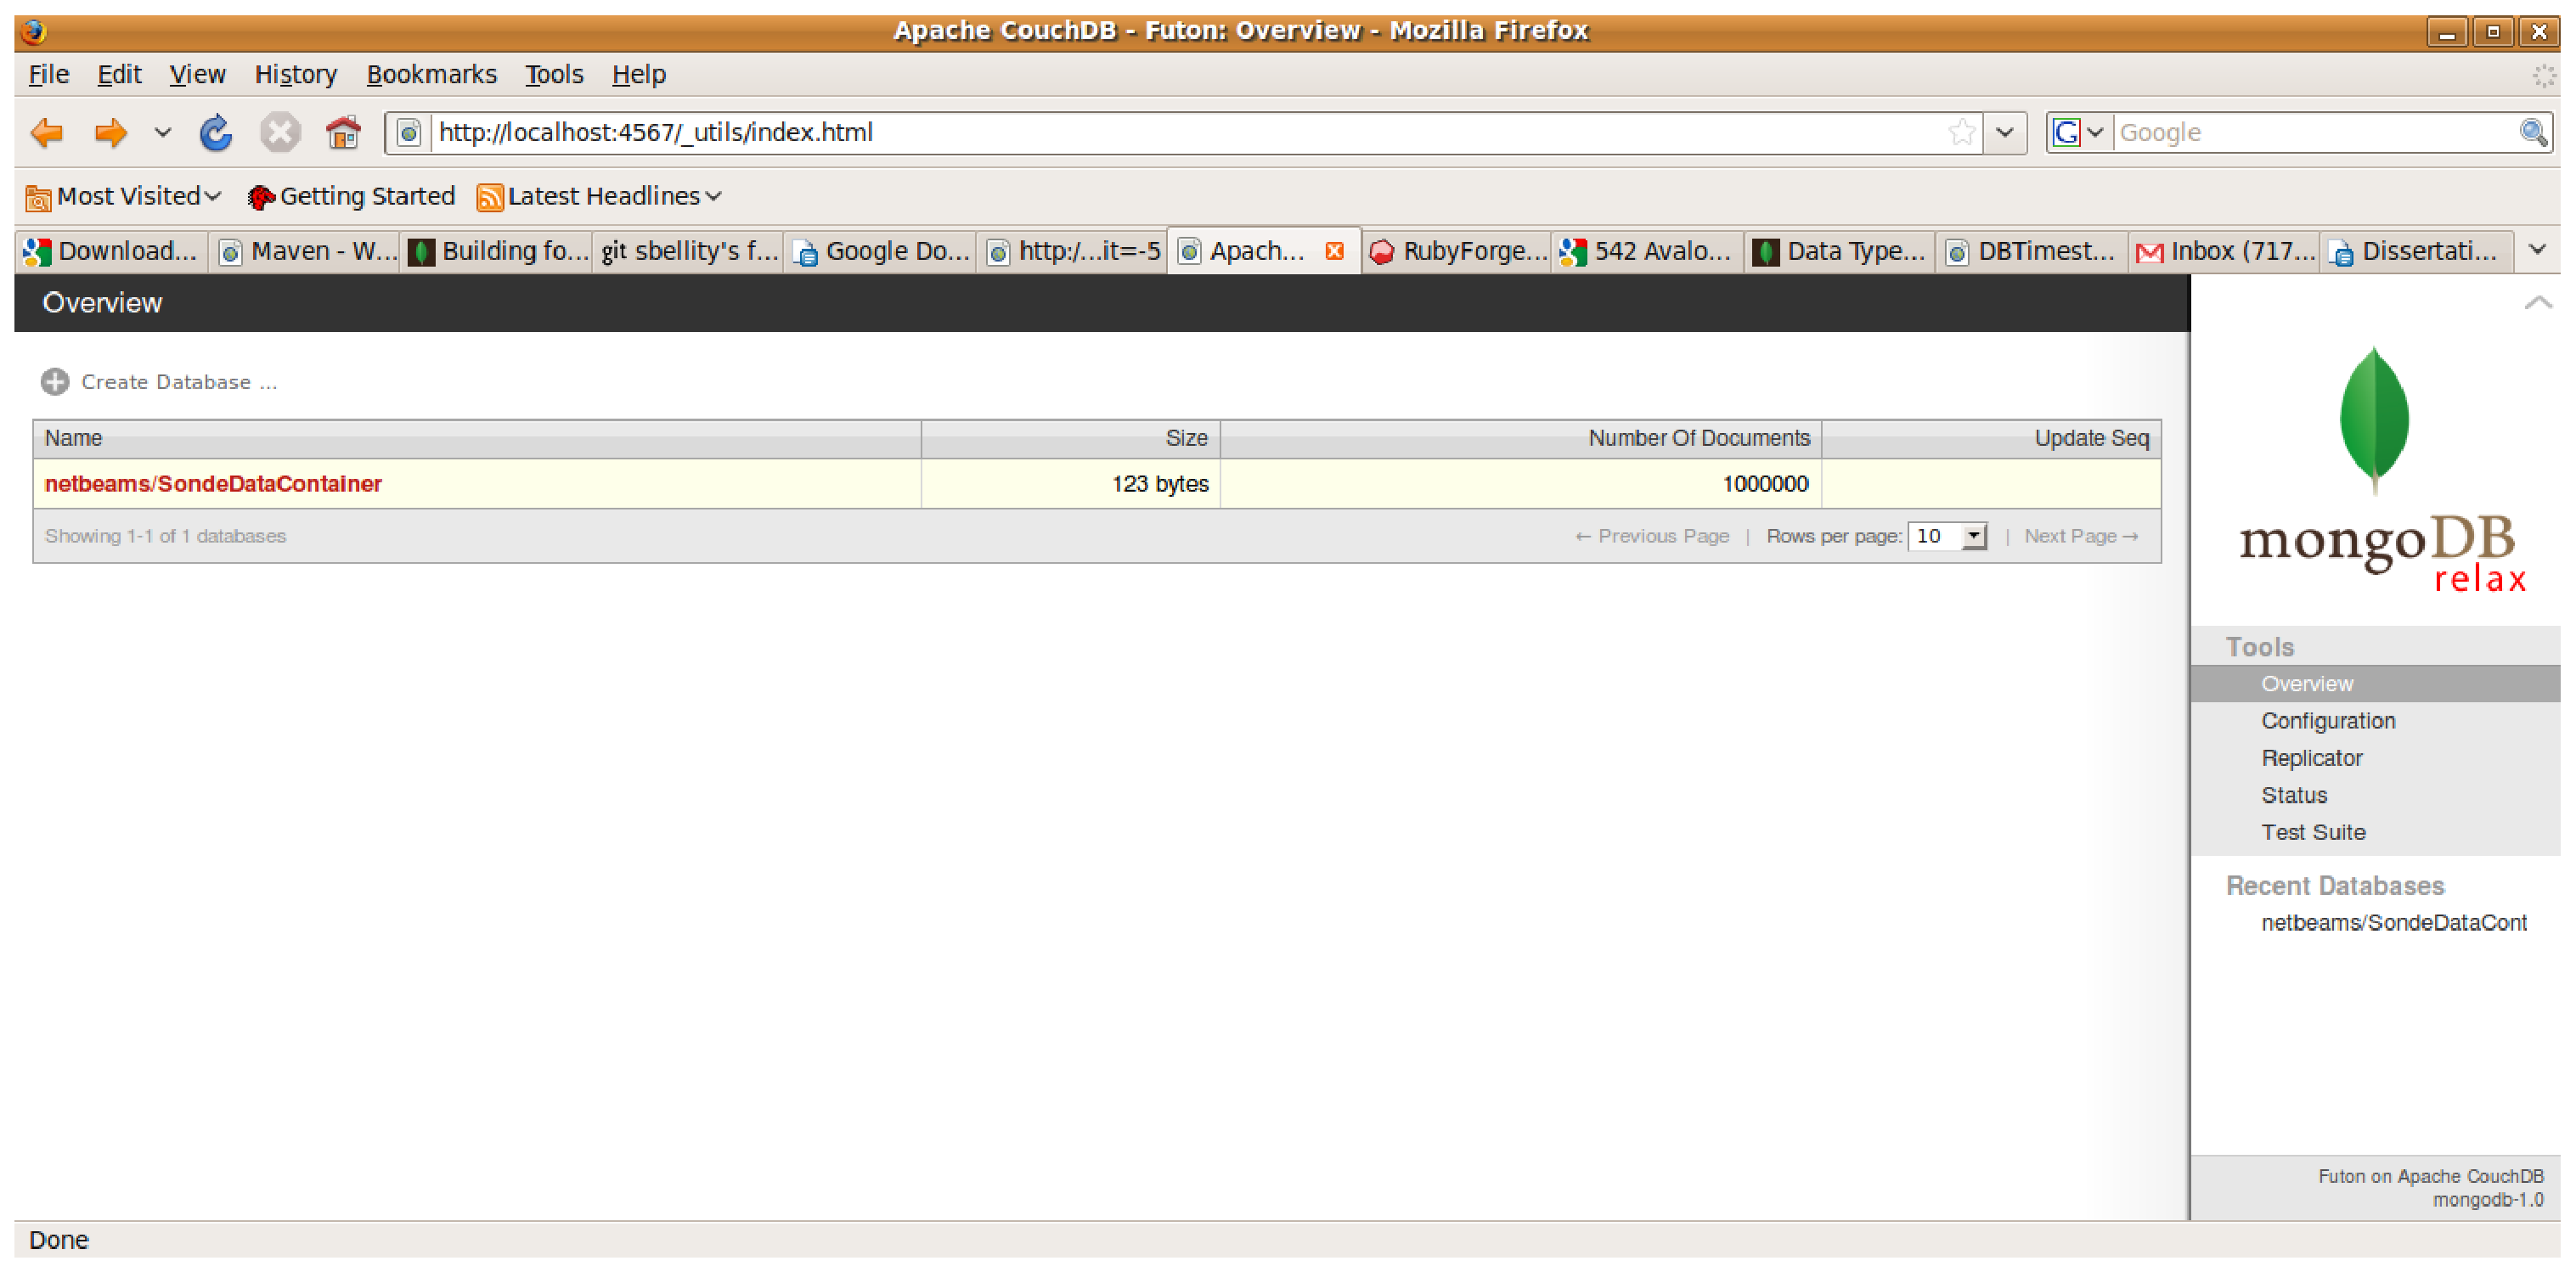
\includegraphics[scale=0.45]{../diagrams/view-collections-instance-browser-futondb}
  \caption{Viewing a partial list of data using the Futon for CouchDB/MongoDB}
  \label{fig:view-collections-instance-browser-futondb}
\end{figure}

The collection is composed by instances of documents of representing the YSI
Sonde type, being indexed by a document ID and the values being the keys
defined in the previous chapter, as shown in figure
\ref{fig:view-collected-data-list-browser-futondb}.

\begin{figure}[h]
  \centering
 
  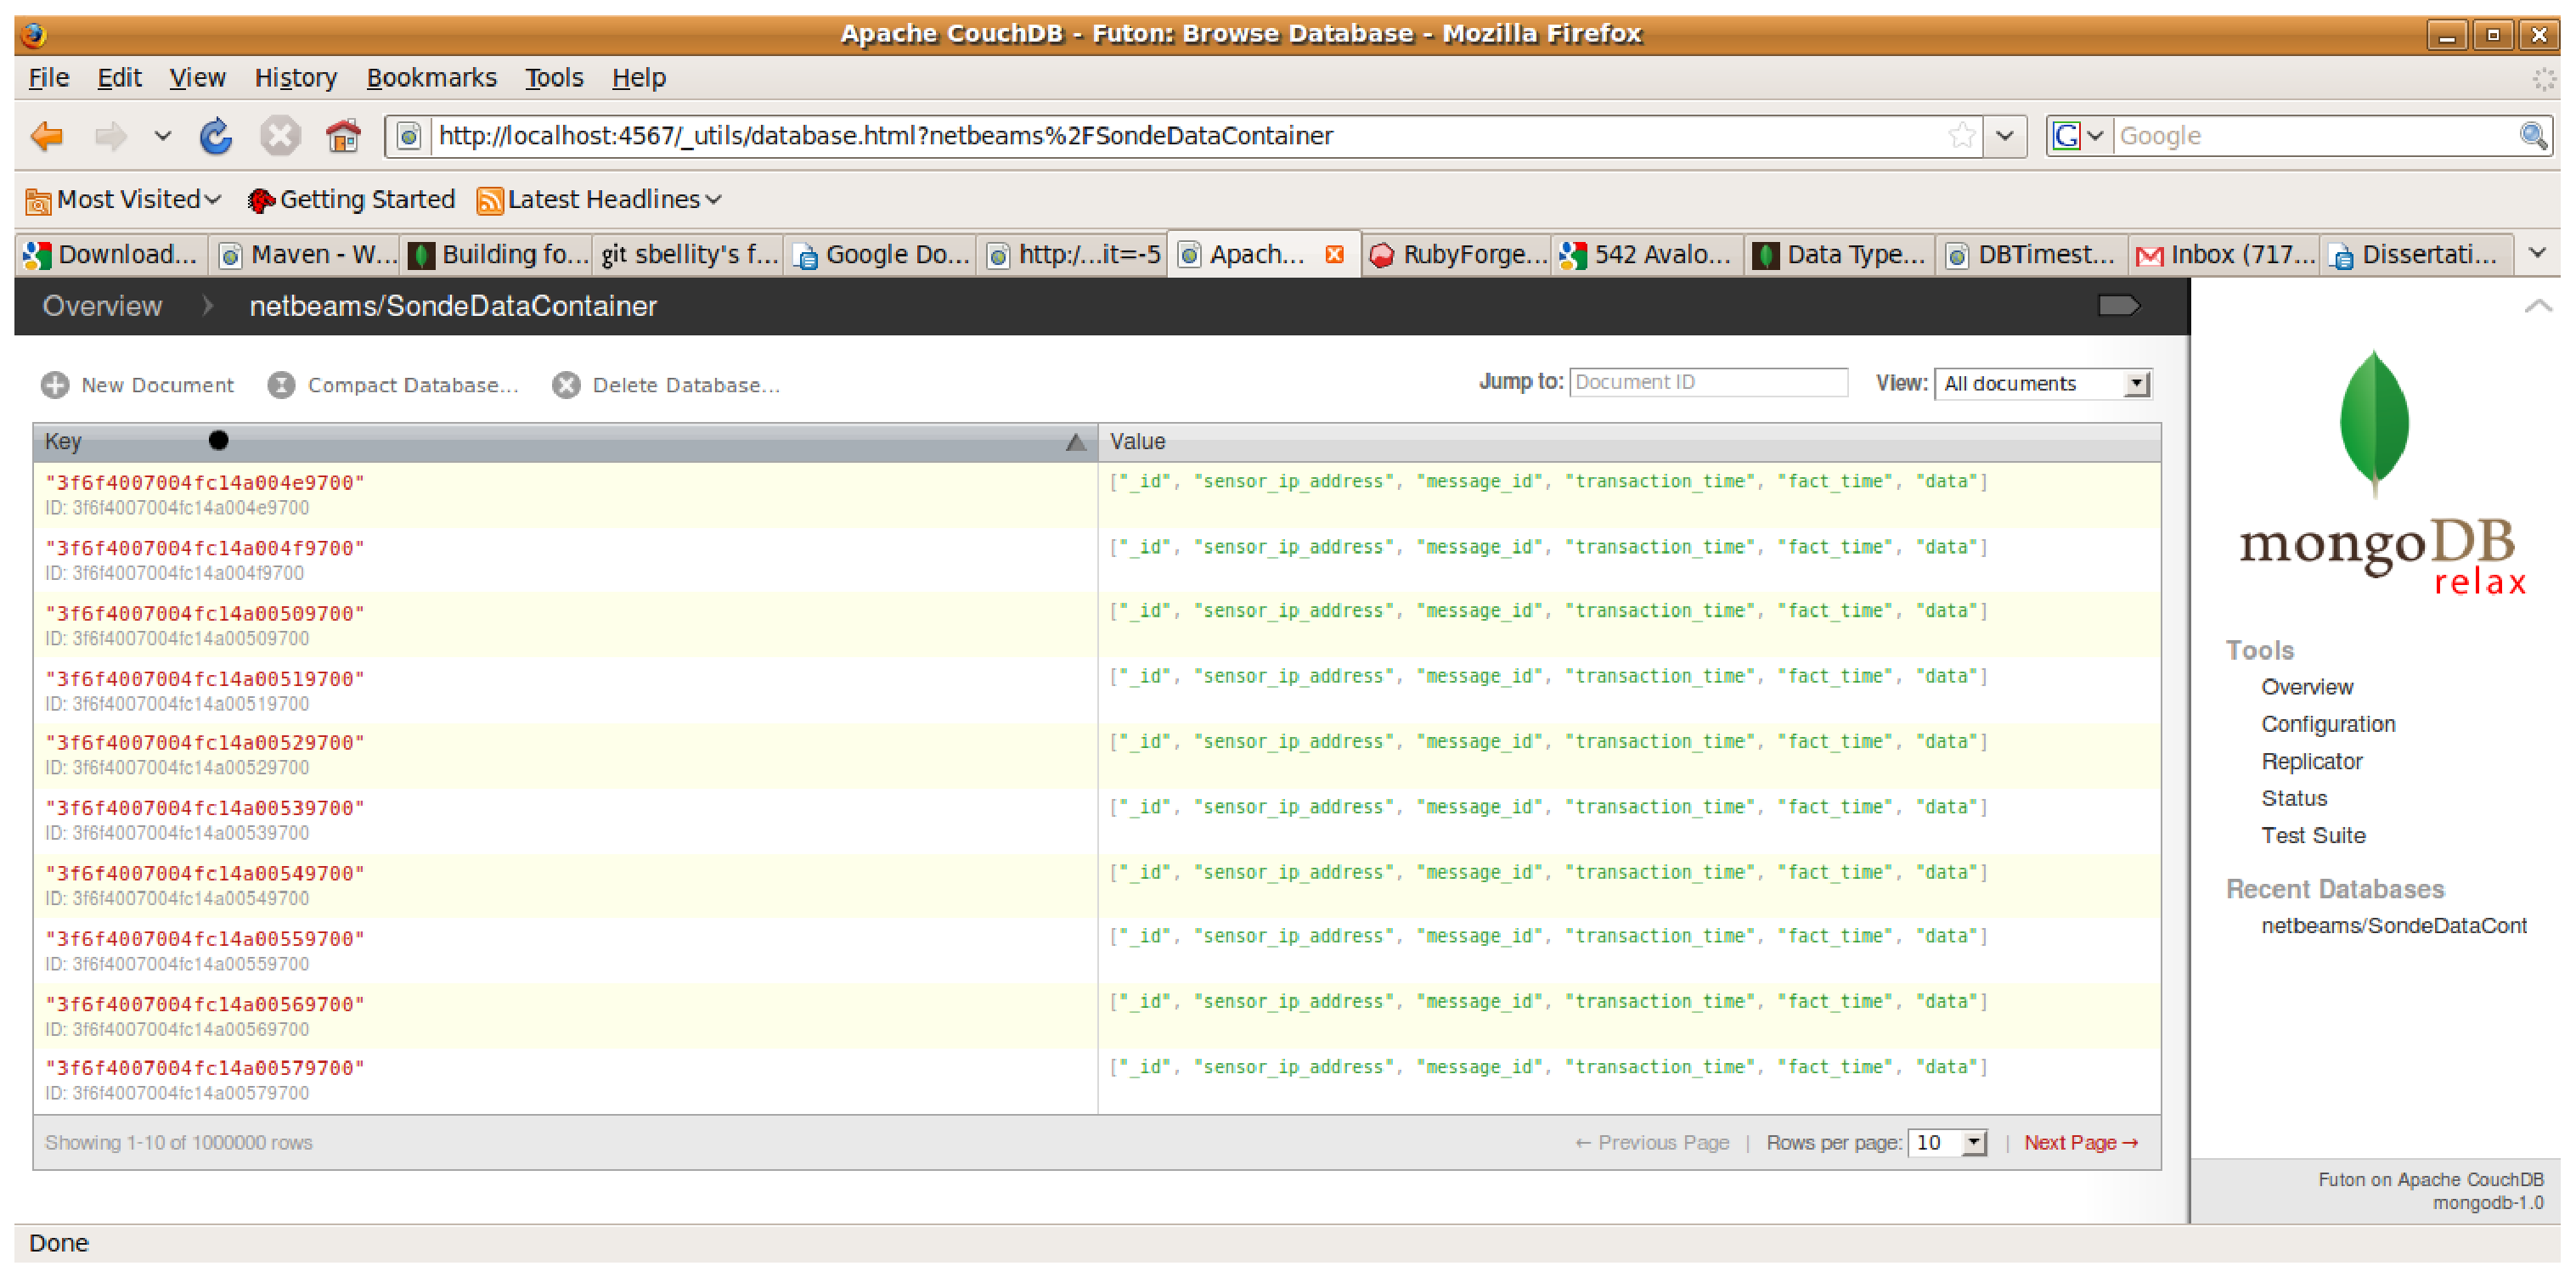
\includegraphics[scale=0.45]{../diagrams/view-collected-data-list-browser-futondb}
  \caption{Viewing a partial list of data using the Futon for CouchDB/MongoDB}
  \label{fig:view-collected-data-list-browser-futondb}
\end{figure}

By clicking in one of the items, one can view the instance of the document, as
it is shown in Figure \ref{fig:view-collections-instance-browser-futondb}.

\begin{figure}[h]
  \centering
  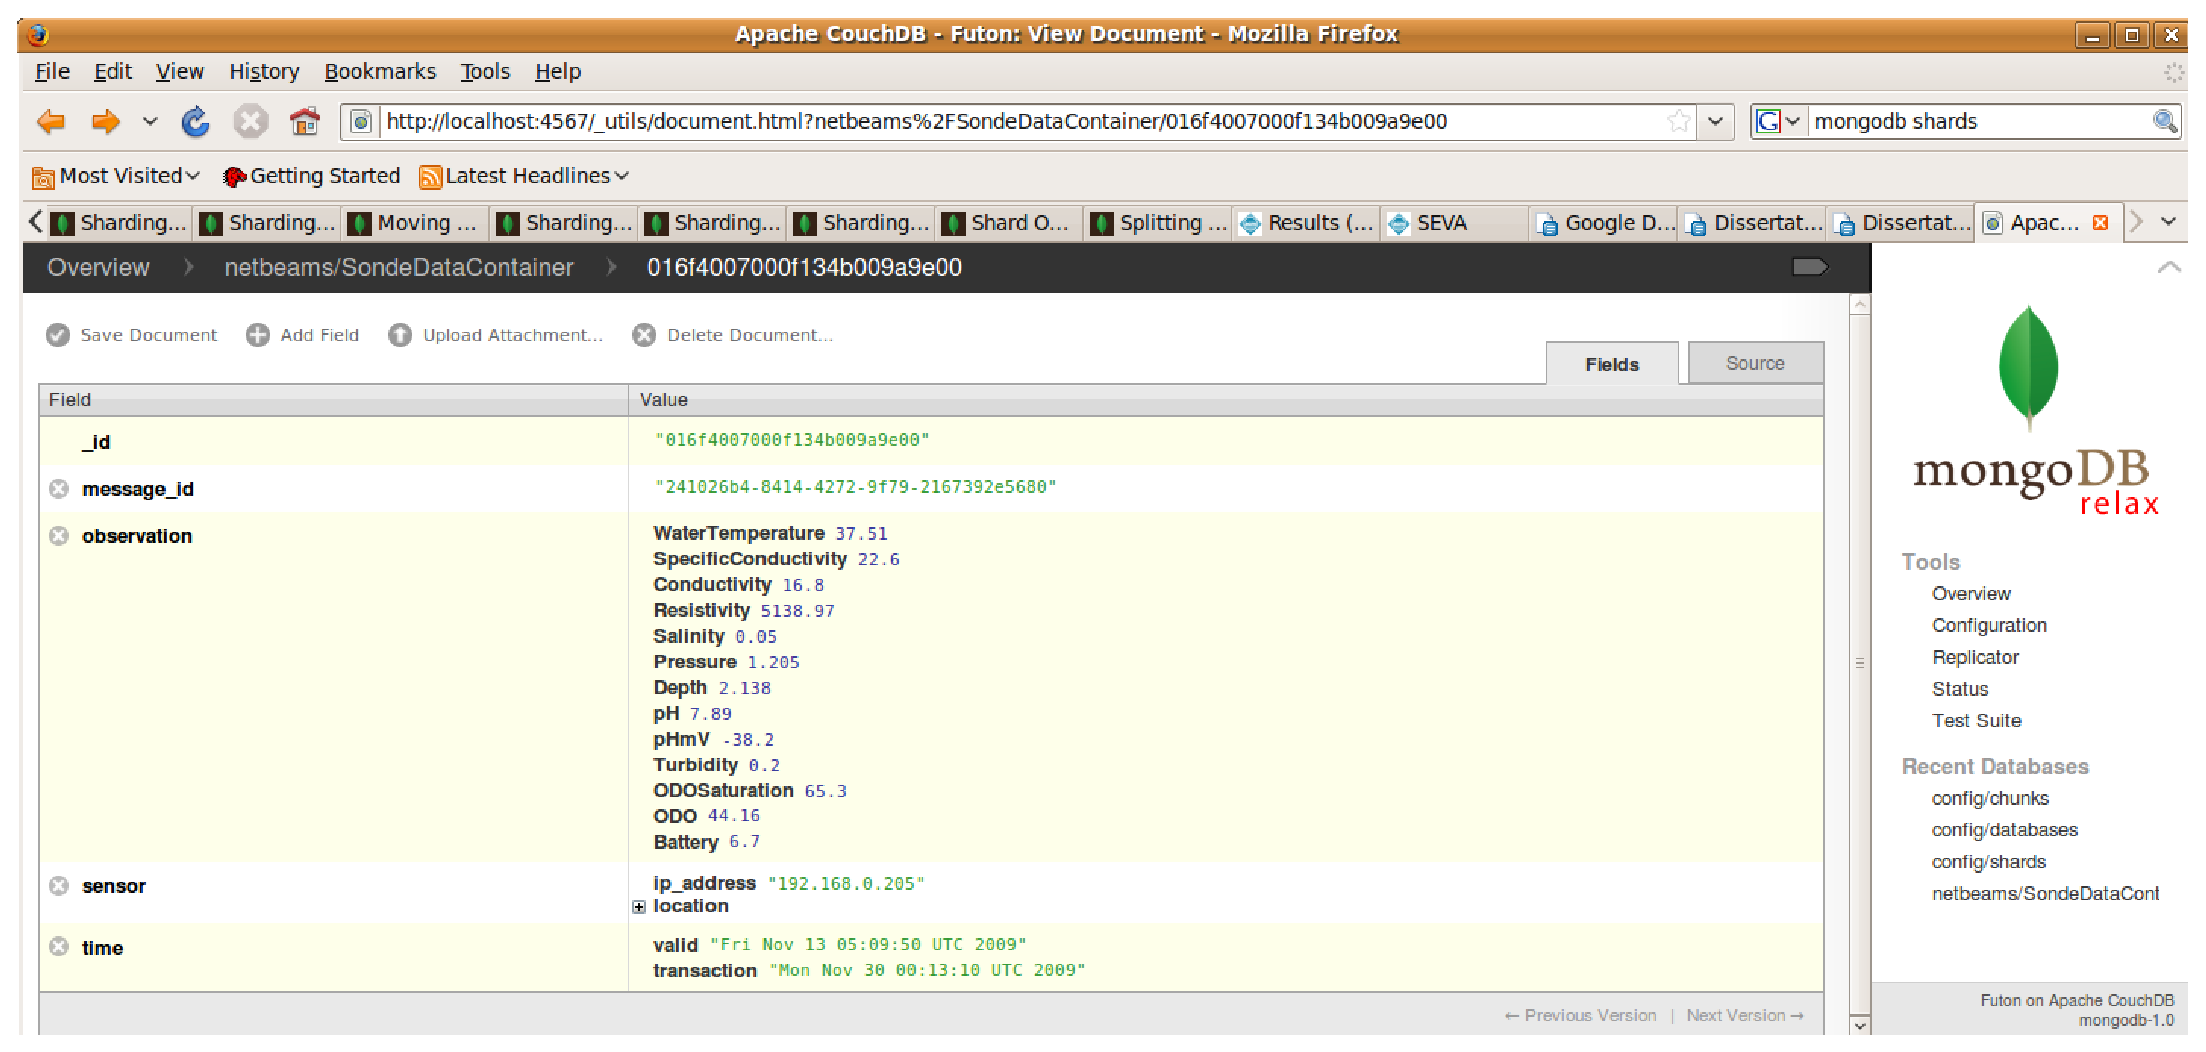
\includegraphics[scale=0.45]{../diagrams/view-collected-data-instance-browser-futondb} \caption{Viewing an instance of collected data using the Futon for CouchDB/MongoDB}
  \label{fig:view-collected-data-instance-browser-futondb}
\end{figure}

\subsection{Exporting Data to Spreadsheets}

mongoDB has an export facility shell called mongoexport. It can export the data
in JSON format or CSV. One may also write its own export tool in any of the
languages such as Java, PHP, Python, Perl, Ruby, among others. A list of the
existing drivers in different languages is provided
athttp://www.mongodb.org/display/DOCS/Drivers. The following command can be
executed to have the exported version of the data in CSV (read the help output
of the command for details).

An example to export the data in CSV format can be seen in listing
\ref{file:mongodb-export-command}, and an example containing 1 million objects can be
downloaded at
http://netbeams.googlecode.com/files/experiment-1000000-data-exported-20090913-053538.csv.tar.gz.

\subsection{Exporting Data to OPeNDAP Format}

By using any programming language driver, one can export data in the OPeNDAP
format.

\section{Source-Code and Implemented Artifacts}

\lstinputlisting[language=Ant,label=file:dsp-build.xml,caption=Build
system using Apache ANT]{../../../../netbeams/versions/v2/apps/osgi-bundles/dsp/DSPDataPersistence/build.xml}

\lstinputlisting[label=file:osgi-intro-manifest,caption=OSGi Manifest
Descriptor]{../../../../netbeams/versions/v2/apps/osgi-bundles/dsp/DSPDataPersistence/META-INF/MANIFEST.MF}

\lstinputlisting[language=XML,label=file:dsp-config.xml,caption=DSP
Deployment
Configuration]{../../../../netbeams/versions/v2/config/deployment/config.xml}

\lstinputlisting[language=XML,label=file:dsp-matcher-config.xml,caption=DSP
Matching Rules]{../../../../netbeams/versions/v2/config/deployment/matcher_config.xml}

\lstinputlisting[language=XML,label=file:dsp-matcher-config-gumstix.xml,caption=DSP
Matching Rules
for
Gumstix]{../../../../netbeams/versions/v2/config/deployment/matcher_config-gumstix.xml}

\lstinputlisting[language=XML,label=file:dsp-data-persistence-bootstrap.xml,caption=DSP
Message used to bootstrap the DSP Data Persistence Component]
{../../../../netbeams/versions/v2/apps/xml/samples/DSPDataPersistence_001.xml}

%TODO: add bootstrap message in case it is implemented

\lstinputlisting[language=Java,label=file:dsp-activator,caption=OSGi
Activator]{../../../../netbeams/versions/v2/apps/osgi-bundles/dsp/DSPDataPersistence/src/org/netbeams/dsp/persistence/osgi/DataPersistenceActivator.java}

\lstinputlisting[language=Java,label=file:dsp-component-service,caption=OSGi
Service - Component]{../../../../netbeams/versions/v2/apps/osgi-bundles/dsp/DSPDataPersistence/src/org/netbeams/dsp/persistence/controller/DSPDataPersistence.java}

\lstinputlisting[language=Java,label=file:dsp-mongo-service,caption=DSP Data to
Mongo DB
Service]{../../../../netbeams/versions/v2/apps/osgi-bundles/dsp/DSPDataPersistence/src/org/netbeams/dsp/persistence/controller/DSPMongoCRUDService.java}

\lstset{language=XML,morecomment=[s]{!--}{--},label=file:dsp-message-serialized-ysi,caption=DSP
Message with a YSI sonde data payload}
\begin{lstlisting}
<?xml version="1.0" encoding="UTF-8" standalone="yes"?>
<MessagesContainer uudi="24929c29-60ee-4d17-af08-64d9446277ef"
        creationTime="2009-03-06T15:17:18-0800" destinationHost="192.168.0.106">
   <MeasureMessage ContentType="org.netbeams.dsp.ysi"
         messageID="435a61f6-370f-458d-aeb7-6e92270a79cb">
      <Header>
         <CreationTime>1236381438480</CreationTime>
         
         <Producer>   
            <ComponentType>
                 org.netbeams.dsp.platform.management.component.ComponentManager
            </ComponentType>
            
            <ComponentLocator>
               <ComponentNodeId>1234</ComponentNodeId>
               <NodeAddress>192.168.0.103</NodeAddress>
            </ComponentLocator>
         </Producer>
         
         <Consumer>
            <ComponentType>
                 org.netbeams.dsp.wiretransport.client
            </ComponentType>
            
            <ComponentLocator>
               <NodeAddress>LOCAL</NodeAddress>
            </ComponentLocator>
         </Consumer>
      </Header>
      <Body>
         <SondeDataContainer>
            <soundeData date="15:17:18" time="03-06-2009">  
               <Temp>21.20</Temp>
               <SpCond>193</SpCond>
               <Cond>179</Cond>
               <Resist>5588.40</Resist>
               <Sal>0.09</Sal>
               <Press>0.084</Press>
               <Depth>0.059</Depth>
               <pH>7.98</pH>
               <phmV>-79.6</phmV>
               <ODOSat>99.5</ODOSat>
               <ODOConc>8.83</ODOConc>
               <Turbid>0.4</Turbid>
               <Battery>8.7</Battery>
            </soundeData>
         </SondeDataContainer>
      </Body>
   </MeasureMessage>
</MessagesContainer>
\end{lstlisting}

\section{Experiment Implementation}

\lstinputlisting[language=Bash,label=file:experiment-setup-executor,caption=Experiment
Main Execution Script]{../../../../netbeams/versions/v2/persistence/run-persistence-experiment}

\lstinputlisting[language=Python,label=file:experiment-setup-mongoshards,caption=Experiment
Main Execution Script]{../../../../netbeams/versions/v2/persistence/setup-mongo-shards.js}

\lstinputlisting[language=Bash,label=file:setup-os-shards-step1,caption=Experiment
Main Execution Script]{../../../../netbeams/versions/v2/persistence/setup-os-shards-step1}

\lstinputlisting[language=Bash,label=file:setup-os-shards-step2,caption=Experiment
Main Execution Script]{../../../../netbeams/versions/v2/persistence/setup-os-shards-step2}

\lstinputlisting[language=Python,label=file:experiment-export-python,caption=Data
Export to from mongoDB to OPEnDAP format.]{../../../../netbeams/versions/v2/persistence/data-export-python.py}

\lstinputlisting[language=Python,label=file:experiment-scenarios,caption=Experiment
Scenarios Implementation]{../../../../netbeams/versions/v2/persistence/experiment-client-scenarios.js}

\lstinputlisting[language=Java,label=file:main-ysi-data-handler,caption=The
DSP YSI Sonde Data Handler]{../../../../netbeams/versions/v2/apps/xml/jaxb/sonde/java-src/org/netbeams/dsp/ysi/SondeDataType.java}

\lstinputlisting[language=Java,label=file:random-ysi-data-generator,caption=Random
Test Data Generator]{../../../../netbeams/versions/v2/apps/osgi-bundles/dsp/DSPSondeProducer/src/org/netbeams/dsp/ysi/SondeTestData.java}

\lstinputlisting[language=Java,label=file:experiment-dsp-java-executor,caption=Inserting
Random Data to MongoDB]{../../../../netbeams/versions/v2/apps/osgi-bundles/dsp/DSPDataPersistence/src/org/netbeams/dsp/persistence/controller/DSPMessageToMongoDBExperiment.java}

\subsection{Experiment Execution Output}

\lstset{label=file:mongodb-ysi-data-format,caption=JSON representation of the
data produced by a YSI sensor on mongoDB}
\begin{lstlisting}
{
    "_id" : ObjectId("5d6f40078ec8074bba980900"),
    "message_id" : "020d82e1-18b2-4fe2-800c-a0f68e22ea86",
    "sensor" : {
        "ip_address" : "192.168.0.91",
        "location" : {
            "latitude" : 37.89155,
            "longitude" : -122.4464
        }
    },
    "time" : {
        "valid" : "Wed Nov 04 2009 02:30:12 GMT-0800 (PST)",
        "transaction" : "Sat Nov 21 2009 03:01:33 GMT-0800 (PST)"
    },
    "observation" : {
        "WaterTemperature" : 88.58,
        "SpecificConductivity" : 180.5,
        "Conductivity" : 167.3,
        "Resistivity" : 491.89,
        "Salinity" : 0.06,
        "Pressure" : 1.109,
        "Depth" : 2.642,
        "pH" : 7.11,
        "pHmV" : -42.9,
        "Turbidity" : 0.2,
        "ODOSaturation" : 72.4,
        "ODO" : 10.85,
        "Battery" : 2.7
    }
}
\end{lstlisting}

\lstset{label=file:rtc-ysi-opendap,caption=HTTP GET Request x Response to the OPeNDAP server at SF-BEAMS}
\begin{lstlisting}
http://sfbeams.sfsu.edu:8080/opendap/sfbeams/data_ctd/rtc_ctd5-ysimoor/real-time/sfb_CTD5_PUF.dat.ascii?
GET /opendap/sfbeams/data_ctd/rtc_ctd5-ysimoor/real-time/sfb_CTD5_PUF.dat.dods?&Month=11&Day=12 HTTP/1.1

HTTP/1.x 200 OK
Server: Apache-Coyote/1.1
Last-Modified: Thu, 12 Nov 2009 17:55:06 GMT
XDODS-Server: Server-Version-Unknown
XOPeNDAP-Server: bes/3.5.1 freeform_handler/3.7.5, netcdf_handler/3.7.6
XDAP: 3.2
Content-Description: dods_data
Content-Type: text/txt
Date: Sun, 15 Nov 2009 03:08:45 GMT

Dataset: sfb_CTD5_PUF.dat
YSI_REALTIME_CSV.Month, YSI_REALTIME_CSV.Day, YSI_REALTIME_CSV.Year, YSI_REALTIME_CSV.Hour, YSI_REALTIME_CSV.Min, YSI_REALTIME_CSV.Sec, YSI_REALTIME_CSV.WaterTemperature, YSI_REALTIME_CSV.SpecificConductivity, YSI_REALTIME_CSV.Conductivity, YSI_REALTIME_CSV.Resistivity, YSI_REALTIME_CSV.TDS, YSI_REALTIME_CSV.Salinity, YSI_REALTIME_CSV.Pressure, YSI_REALTIME_CSV.Depth, YSI_REALTIME_CSV.pH, YSI_REALTIME_CSV.pHmV, YSI_REALTIME_CSV.Turbidity, YSI_REALTIME_CSV.ODOSaturation, YSI_REALTIME_CSV.ODO, YSI_REALTIME_CSV.Chlor, YSI_REALTIME_CSV.Chlor_RFU, YSI_REALTIME_CSV.Battery, YSI_REALTIME_CSV.InstSN
11, 12, 2009, 16, 30, 51, 13.78, 4.3945, 3.4532, 0, 28.56, 28.35, 2.65, 2.651, 7.9, -54.7, 9, -99999, -99999, 3.7, 1, 9.4, -99999
11, 12, 2009, 16, 36, 50, 13.78, 4.4095, 3.4642, 0, 28.66, 28.46, 2.628, 2.63, 7.91, -54.9, 11.9, -99999, -99999, 4, 1.1, 9.4, -99999
11, 12, 2009, 16, 42, 51, 13.77, 4.3943, 3.4515, 0, 28.56, 28.35, 2.631, 2.632, 7.9, -54.9, 9.8, -99999, -99999, 3.6, 1, 9.4, -99999
11, 12, 2009, 16, 48, 50, 13.76, 4.3893, 3.447, 0, 28.53, 28.32, 2.628, 2.63, 7.9, -54.8, 10.6, -99999, -99999, 3.8, 1, 9.4, -99999
\end{lstlisting}

\lstset{label=file:mongodb-export-command,caption=Export Command to CSV format}
\begin{lstlisting}
mongoexport -d netbeams -c SondeDataContainer --dbpath data --csv -f "_id,sensor_ip_address,transaction_time,fact_time,data.temperature,data.sp_condition,data.condition,data.resistence,data.salinitude,data.pressure,data.depth,data.ph,data.pH_mv,data.odo_sat,data.odo_condition,data.turbidity,data.battery" -o logs/experiment-483840-data-exported-20091129-190207.csv

Sun Nov 29 19:07:04 query netbeams.SondeDataContainer ntoreturn:0 reslen:2258 nscanned:101 { query: {}, $snapshot: 1 }  nreturned:101 202ms
Sun Nov 29 19:07:04 getmore netbeams.SondeDataContainer cid:7749363894863150628 ntoreturn:0 query: { query: {}, $snapshot: 1 }  bytes:1048562 nreturned:47661 1767ms
...
...
Sun Nov 29 19:10:18 getmore netbeams.SondeDataContainer cid:7749363894863150628 ntoreturn:0 query: { query: {}, $snapshot: 1 }  bytes:793098 nreturned:36049 1975ms
exported 2419200 records
\end{lstlisting}

\lstinputlisting[label=file:experiment-export-python-results,caption=Data
Export to from mongoDB to OPEnDAP format.]{../../../../netbeams/versions/v2/persistence/export-mongodb-to-sfbeams.csv}

\begin{figure}[h]
  \centering
  \includegraphics[scale=0.4]{../diagrams/experiment-mouseactions-dsp}
  \caption{Experiment showing the mongoDB persisting messages from the DSP
  Mouse Actions Demo}
  \label{fig:experiment-mouseactions-dsp}
\end{figure}